\chapter{模擬與評估系統表現}
\label{chp:4}


第三章中,我們提出了一個多LED對多PD系統的演算法,在不需限制目標平面與使用者平面平行的情況下,具有獲得三維定位以及目標物姿態的能力,而在硬體擺放的指向以及數量上也具有靈活度,而本章節的主要目的便是希望探討不同系統設計對定位的影響。為了評估不同系統設計,我們需要利用硬體驗證或是軟體模擬的方法,完成完整的定位系統流程(參考圖\ref{pic:lp_system_flow}),以進行定位誤差的計算與評估。

\begin{figure}[ht]
    \centering
    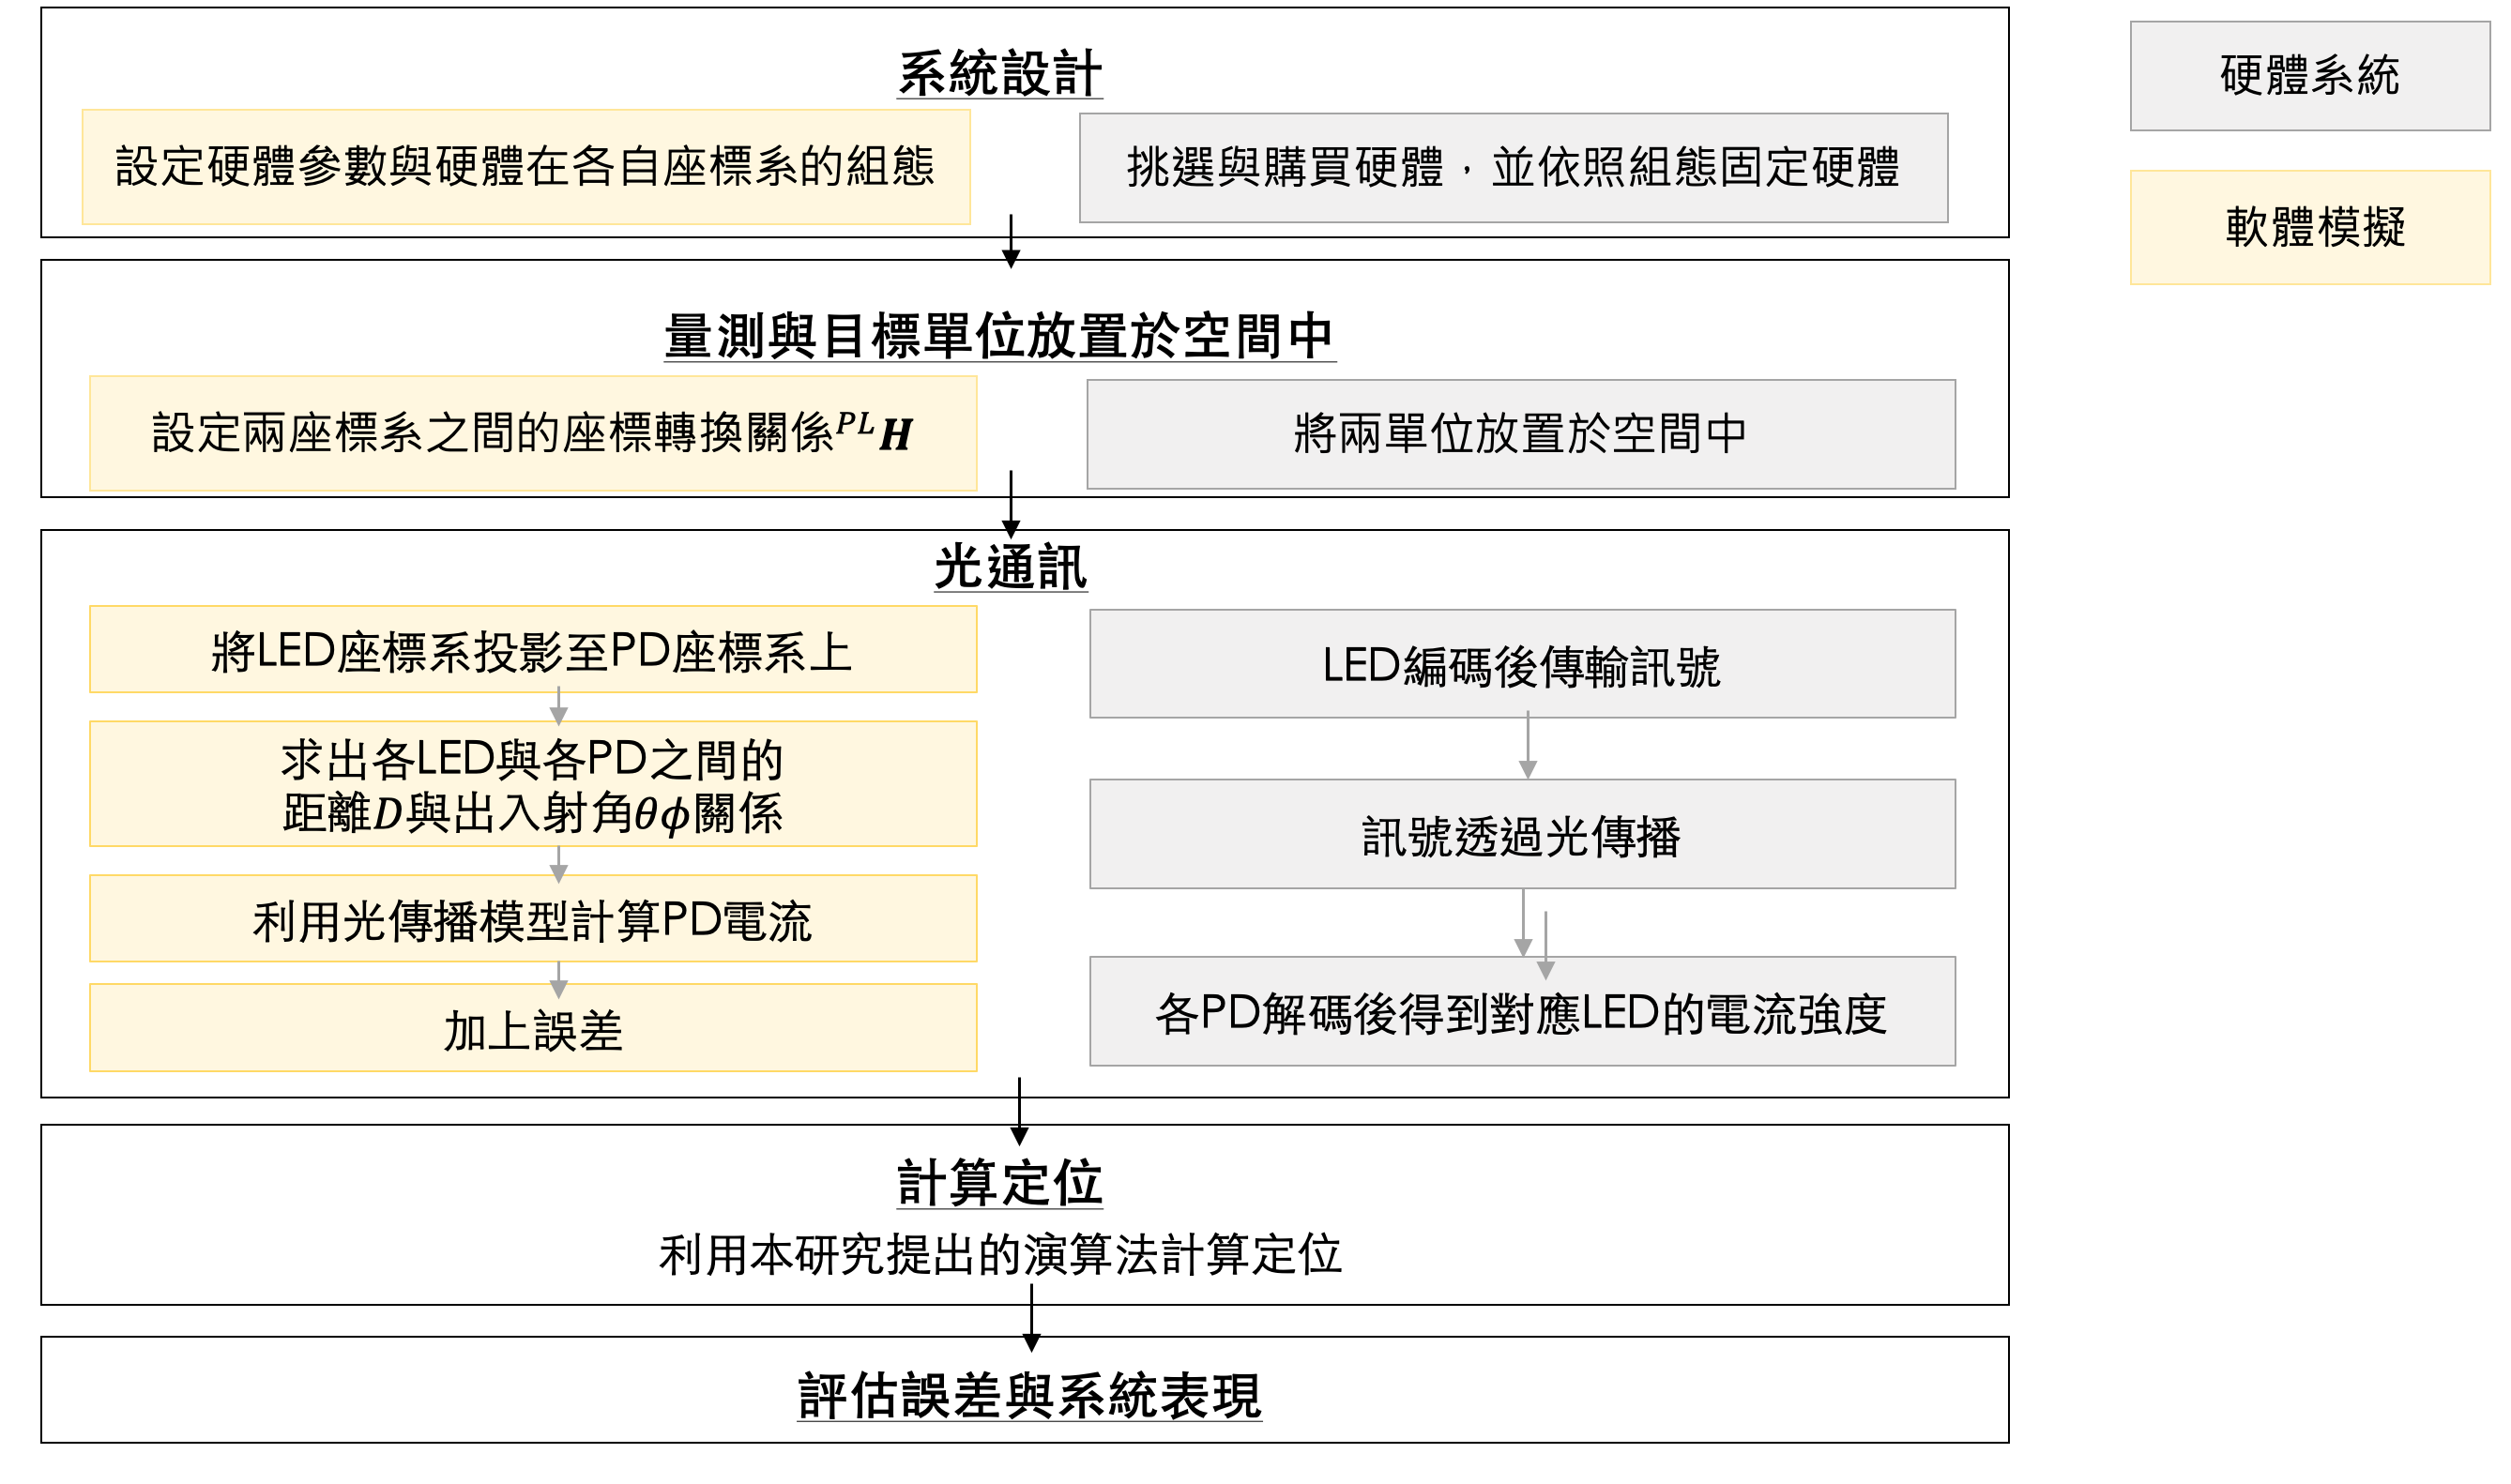
\includegraphics[width=15cm]{ch4pic/simulate_hardware.png}
    \caption{多LED對多PD定位系統以硬體驗證與軟體模擬的流程圖}
    \label{pic:simulate_hardware}
\end{figure}

參考圖\ref{pic:simulate_hardware},硬體驗證的方法會由挑選硬體以及設計硬體模組開始,在硬體系統搭建完成後,將兩硬體單位放置於量測位置,透過光通訊的技術得到各LED對各PD的電流強度。軟體模擬的部分,則是以數學方式描述硬體參數、硬體組態、以及兩座標系之間的轉換關係,並以光傳遞模型來模擬光通訊所得到的硬體輸出電流。比較硬體與軟體模擬的特性, 最完整的驗證方法為硬體驗證,然而由於光通訊發展並不如無線電波段成熟,架設光通訊系統較不方便,因此硬體驗證的複雜度較高;除此之外,硬體購買以及設計硬體模組的部分,都需要花費時間與金錢成本進行架設,在調整系統設計上也不如軟體靈活。也因此,大多數的文獻上會先透過軟體模擬,評估系統與演算法的表現,藉由低成本又快速方便的軟體模擬,在實際搭建硬體系統之前先對該設計有所了解,以做為硬體系統設計的參考。

因此,本論文會利用軟體模擬的方法,建立一模擬環境,將光通訊的步驟在模擬中完成,再以第三章提出的定位演算法計算出相對位置,並評估誤差與系統表現。以下依序在\ref{chp:simulation}章中詳細介紹如何透過數學模型模擬實際情況,而我們將數值帶入模擬方法得到的結果呈現於\ref{chp:simulate_result},於\ref{chp:system_evaluate}章中則對不同的系統設計進行分析以及評估,最後於\ref{chp:4_conclusion}章中總結。


\section{模擬方法}
\label{chp:simulation}

根據圖\ref{pic:simulate_hardware}中軟體模擬的流程,本章節由\ref{chp:system_design}章中介紹軟體模擬中的系統設計,於\ref{chp:simulate_position}章中模擬兩硬體單位於不同位置的擺放,於\ref{chp:simulate_vlc}章中模擬光通訊的硬體輸出訊號,而透過第三章提出的演算法得到的模擬定位結果則呈現於\ref{chp:simulate_result}章。




\subsection{系統設計模擬}
\label{chp:system_design}

系統設計中,我們需決定硬體數量$L,P$,以及硬體的規格與組態,在此章節將敘述軟體模擬中需設定的數值,以及與實際硬體系統設計時的差異。

\subsubsection{硬體數量}

硬體數量的部分,參考\ref{chp:orient_conclu}章中所述,LED與PD數量各需要最少三個來達成三維定位,因此在設定數量$L,P$時需確定其大於等於3,參考表\ref{tab:para_amount}。

\begin{table}[h]
    % \toprule% you can only use this within a tabular and if you load booktabs
    \renewcommand{\arraystretch}{1.3}
    \setlength{\arrayrulewidth}{0.15mm}
    \setlength{\doublerulesep}{0.12mm}
    \caption{模擬中需設定的硬體數量}
    \label{tab:para_amount}
    \centering
    \begin{tabular}{|cc|c|c|}
    \hline
    \multicolumn{2}{|c|}{\textbf{硬體數量}}  &\textbf{單位}  &  \textbf{備註}   \\
    \hline
     LED數量 &$L$ & 個 & 最小為3的整數 \\\hline
      PD數量& $P$& 個  & 最小為3的整數 \\\hline
    \end{tabular}
\end{table}
    
\subsubsection{硬體參數}

硬體規格在挑選時需著重注意的參數可以參考圖\ref{pic:hardware_para},包含影響輻射模式的朗博次方$Mp,M\ell$
,以及影響收發光強度的參數:LED總輻射通量$Pt$、PD有效面積$A$、飽和電流$s$、響應率$Re$;我們將這些參數統整於表\ref{tab:para_hardware}。這些參數中,除了朗博次方$M\ell,Mp$與有效面積$A$以外,各參數又會隨著給予的電壓電流改變。因此,\textbf{挑選朗博次方格外重要},一旦購買該規格硬體則無法調整輻射模型,不像其他可在購買後透過提高給定電壓電流來提升表現。

需要注意的是,朗博輻射模型在軟體模擬中,可以設定為任意大於一的數值,設計空間為連續的;然而實際硬體挑選時,各硬體的朗博次方無法改變,設計空間不連續,僅能從市面上的硬體中挑選合適的,在市售硬體中無法指定所需的朗博次方。

\begin{table}[h]
% \toprule% you can only use this within a tabular and if you load booktabs
\renewcommand{\arraystretch}{1.3}
\setlength{\arrayrulewidth}{0.15mm}
\setlength{\doublerulesep}{0.12mm}
\caption{模擬中需設定的硬體參數}
\label{tab:para_hardware}
\centering
\begin{tabular}{|c|cc|c|c|}
\hline
\multicolumn{3}{|c|}{\textbf{硬體參數}}  &\textbf{單位}  &  \textbf{備註}   \\
\hline
\multirow{2}{*}{LED} 
& 總輻射通量 &$Pt$ & $W/sr$ & 可透過改變電壓調整 \\
 & 朗博次方& $M\ell$& -  & 最小為1 \\\hline
\multirow{4}{*}{PD} 
& 響應率 &$Re$ & $A/W$ & 可透過改變電壓調整 \\
& 有效面積& $A$& $m^2$ & - \\
& 飽和電流& $s$& $A$ & 可透過改變電壓調整 \\
& 朗博次方& $Mp$& -  & 最小為1 \\\hline
\end{tabular}
\end{table}



\subsubsection{硬體組態}

硬體組態的部分,位置的限制如\ref{chp:algorithm_constraint}章中所述,需限制PD擺放位置於PD座標系原點:$^P\boldsymbol{P}_p=
\left[\begin{array}{ccc}0&0&0\end{array}\right]^T$,LED的擺放位置也限制於LED座標系原點:$^L\boldsymbol{P}_l=
\left[\begin{array}{ccc}0&0&0\end{array}\right]^T$。而實際在設計硬體模組時,可以參考圖\ref{pic:ml_pd_config},需要將各電子元件與LED、PD硬體固定於一特殊形狀的載體上,利用載體的形狀來調整硬體的擺放指向。在模擬時,我們僅需透過定義各硬體的指向$\boldsymbol{V}$即可,其中各指向有兩個自由度:以球座標系定義的天頂角$\alpha$與方位角$\beta$。改變各硬體的指向時,各硬體的照射範圍也會改變,導致定位效果不同,因此硬體指向如何設計為一影響系統表現的因素,於\ref{chp:evaluate}章中進行評估。執得注意的是,每一個硬體的組態需要定義兩個自由度,因此組態的部分,總共需定義$2\times(L+P)$個自由度,組態的變數數量為硬體數量的函數。

\begin{table}[h]
    % \toprule% you can only use this within a tabular and if you load booktabs
    \renewcommand{\arraystretch}{1.3}
    \setlength{\arrayrulewidth}{0.15mm}
    \setlength{\doublerulesep}{0.12mm}
    \caption{模擬中需設定的硬體組態}
    \label{tab:para_config}
    \centering
    \begin{tabular}{|c|cc|c|c|}
    \hline
    \multicolumn{3}{|c|}{\textbf{組態參數}}  &\textbf{單位}  &  \textbf{備註}   \\
    \hline
    \multirow{2}{*}{第$l$個LED} 
    & 天頂角 &$^L \alpha_l$ & $rad$ & $0\leq ^L \alpha_l<\pi$ \\
     & 方位角& $^L \beta_l$& $rad$ & $0\leq ^L \beta_l<2\pi$ \\\hline
    \multirow{2}{*}{第$p$個PD} 
    & 天頂角 &$^P \alpha_p$ & $rad$ & $0\leq ^P \alpha_p<\pi$ \\
    & 方位角& $^P \beta_p$& $rad$ & $0\leq ^P \beta_p<2\pi$ \\\hline
    \end{tabular}
    \end{table}
    

\subsection{兩硬體單位擺放位置的模擬}
\label{chp:simulate_position}



根據\ref{chp:LEDPD_flow}章中描述,LED與PD各自可視為一個座標系,而兩者之間的相對關係可以齊次座標轉換表示,參考\ref{chp:relative}章。因此,我們可以透過改變齊次轉換矩陣$^{PL}\boldsymbol{H}$,使兩座標系之間的相對關係改變,以模擬兩硬體單位於空間中擺放位置。

而根據式\ref{eqn:homogeneous}中呈現,齊次座標轉換矩陣$^{PL}\boldsymbol{H}$可以視為平移向量$^{PL}\boldsymbol{T}$與旋轉矩陣$^{PL}\boldsymbol{Ro}$綜合的效果,而平移與旋轉各自三個自由度,呈現於表\ref{tab:para_relative}。我們透過定義平移矩陣與旋轉矩陣來模擬兩硬體單位於空間中的相對位置,如式\ref{eqn:simulate_position},平移位置透過$^{PL}t_x,^{PL}t_y,^{PL}t_z$三項定義,而旋轉則透過翻滾角$^{PL}rx$(Roll)、俯仰角$^{PL}ry$(Pitch)、偏航角$^{PL}rz$(Yaw)定義,各自代表繞x,y,z軸旋轉的角度,則旋轉矩陣可以寫為$^{PL}\boldsymbol{Rx},^{PL}\boldsymbol{Ry},^{PL}\boldsymbol{Rz}$三個矩陣的相乘結果。

\begin{equation}
    \label{eqn:simulate_position}
    \begin{aligned}
    ^{PL}\boldsymbol{T} &= 
    \left[\begin{array}{c}
        ^{PL}t_x \\^{PL}t_y\\^{PL}t_z
    \end{array}\right]\\
    ^{PL}\boldsymbol{Ro} &= 
    ^{PL}\boldsymbol{Rz} (^{PL}rz)^{PL}\boldsymbol{Ry}(^{PL}ry) ^{PL}\boldsymbol{Rx} (^{PL}rx)\\
    \text{Where }&\\
    &^{PL}\boldsymbol{Rx} (^{PL}rx) =
    \left[ \begin{array}{ccc}
        1&0&0\\
        0&\cos (^{PL}rx) &-\sin (^{PL}rx) \\
        0&\sin (^{PL}rx) &\cos (^{PL}rx) 
    \end{array}\right] \\
    &^{PL}\boldsymbol{Ry}(^{PL}ry)=
    \left[ \begin{array}{ccc}
        \cos (^{PL}ry) &0&\sin (^{PL}ry) \\
        0&1&0\\
        -\sin (^{PL}ry) &0&\cos (^{PL}ry)
    \end{array}\right]\\
    &^{PL}\boldsymbol{Rz} (^{PL}rz) = 
    \left[ \begin{array}{ccc}
        \cos (^{PL}rz) &-\sin (^{PL}rz)& 0 \\
        \sin (^{PL}rz) &\cos (^{PL}rz)& 0 \\
        0 &0&1
    \end{array}\right]\\
    \end{aligned}
\end{equation}

\begin{table}[h]
    % \toprule% you can only use this within a tabular and if you load booktabs
    \renewcommand{\arraystretch}{1.3}
    \setlength{\arrayrulewidth}{0.15mm}
    \setlength{\doublerulesep}{0.12mm}
    \caption{模擬中定義相對位置的參數}
    \label{tab:para_relative}
    \centering
    \begin{tabular}{|c|cc|c|c|}
    \hline
    \multicolumn{3}{|c|}{\textbf{定義相對位置的參數}}  &\textbf{單位}  &  \textbf{備註}   \\
    \hline
    \multirow{3}{*}{平移向量$^{PL}\boldsymbol{T}$自由度} 
    & x分量 &$^{PL}t_x$ & $m$ &  \\
    & y分量 &$^{PL}t_y$ & $m$ &  \\
    & z分量 &$^{PL}t_z$ & $m$ &  \\
    \hline
    \multirow{3}{*}{旋轉矩陣$^{PL}\boldsymbol{Ro}$自由度} 
    & Roll &${^{PL}rx}$ & $rad$ &  $0\leq {^{PL}rx}<2\pi$\\
    & Pitch &$^{PL}ry$ & $rad$ & $0\leq {^{PL}rx}<2\pi$ \\
    & Yaw &$^{PL}rz$ & $rad$ & $0\leq {^{PL}rx}<2\pi$ \\
    \hline
    \end{tabular}
    \end{table}

\subsection{光通訊訊號模擬}
\label{chp:simulate_vlc}

    理想的光通訊訊號強度,可以藉由光傳遞模型(式\ref{eqn:model_coor_extend})描述,透過將硬體參數、硬體組態與兩座標系相對位置帶入,即可計算出理想的PD電流輸出$Ie_{lp}$。然而實際情況下,硬體量測具有誤差,因此我們參考大多文獻模擬誤差的方式,呈現於\ref{chp:hardware_error}章中。

    \subsubsection{模擬硬體誤差}
    \label{chp:hardware_error}

    圖\ref{pic:simulate_hardware}流程中,模擬光通訊的部分可透過式\ref{eqn:model_algorithm_filter}獲得,而為了更真實的模擬現實狀況,參考\cite{survey_light2018}中對誤差的模擬,呈現於式\ref{eqn:noise}中,$\hat{Ie}_{lp}$代表第l個LED對第p個PD的量測電流,其組成包含了理想的量測電流$Ie_{lp}$與PD硬體誤差。PD硬體誤差中,又可分為熱雜訊$It$(Thermal Noise)與散粒雜訊$Is$(Shot Noise),各自呈現於式\ref{eqn:thermal_noise}與式\ref{eqn:shot_noise}中,其中$Kb$為波茲曼常數(Boltzmann constant)、$Te$為絕對溫度、$B$為頻寬、$Rs$為分路電阻(Shunt Resistance)、$q$為電子電荷。

    \begin{equation}
    \label{eqn:noise}
        \hat{Ie}_{lp}=Ie_{lp}+\sqrt{It_{lp}^2+Is_{lp}^2} 
    \end{equation}


    \begin{gather}
        \label{eqn:thermal_noise}
        It_{lp}=\sqrt{\frac{4 Kb Te B}{Rs}}\\
        \label{eqn:shot_noise}
        Is_{lp}=\sqrt{2qIe_{lp}B}
    \end{gather}

    除了加上誤差以外,我還需評估硬體的解析度,光電二極體的解析度可以用雜訊等效功率(noise equivalent power,以下簡稱NEP)描述,在模擬訊號時的解析度以NEP決定,而NEP大小則取自硬體規格表。

    模擬硬體誤差這段落所需設定得參數整理於表\ref{tab:para:error}:

    \begin{table}[h]
        % \toprule% you can only use this within a tabular and if you load booktabs
        \renewcommand{\arraystretch}{1.3}
        \setlength{\arrayrulewidth}{0.15mm}
        \setlength{\doublerulesep}{0.12mm}
        \caption{模擬硬體誤差需定義的參數}
        \label{tab:para_error}
        \centering
        \begin{tabular}{|cc|c|c|}
        \hline
        \multicolumn{2}{|c|}{\textbf{模擬硬體誤差的參數}}  &\textbf{單位}  &  \textbf{備註}   \\
        \hline
        絕對溫度 &$Te$ & $K$ &  \\
        頻寬 &$B$ & $Hz$ &  \\
        分路電阻 &$Rs$ & $\Omega$ &  \\
        雜訊等效功率 &$NEP$ & $\Omega$ &  \\
        \hline
        \end{tabular}
    \end{table}


    \subsection{計算定位結果}

    我們將上述的系統設計、相對位置、誤差模擬等以數值帶入模型,透過圖\ref{pic:simulate_hardware}中軟體模擬的流程計算不同系統設計下,兩硬體於空間中各位置的距離與方位。

    有了流程之後,我們即可將欲評估的系統設計與相對位置帶入,利用計算出的定位$ \hat{^{PL}\boldsymbol{T} }$與定義相對位置的平移向量$^{PL}\boldsymbol{T}$,兩之間的歐氏距離作為誤差$\hat{e}$。










\section{計算定位結果}
\label{chp:simulate_result}

上一章介紹了如何使用

在此段落,我們將上述的系統設計、相對位置、誤差模擬等以數值帶入模型,透過圖\ref{pic:simulate_hardware}中軟體模擬的流程計算不同系統設計下,兩硬體於空間中各位置的定位誤差。使用的參數於\ref{chp:simulate_para}章中紀錄,而模擬的結果呈現於\ref{chp:simulate_result_sub}章中。

\subsection{使用參數}
\label{chp:simulate_para}

硬體選擇市面上可以購置的作為參考

誤差模擬的方法,根據誰的說法,背景光源誤差影響大,bandwidth參考誰


飽和ˊ

\subsection{模擬結果}
\label{chp:simulate_result_sub}

根據上述的系統設計與誤差模擬方法,我們將兩座標系至於模擬空間中,定義齊次座標轉換矩陣為

結果如下



我們參考文獻最常見的使用情境,將座標於空間中移動,誤差大小以顏色呈現於圖










\section{系統評估}
\label{chp:evaluate}



\begin{figure}[ht]
    \centering
    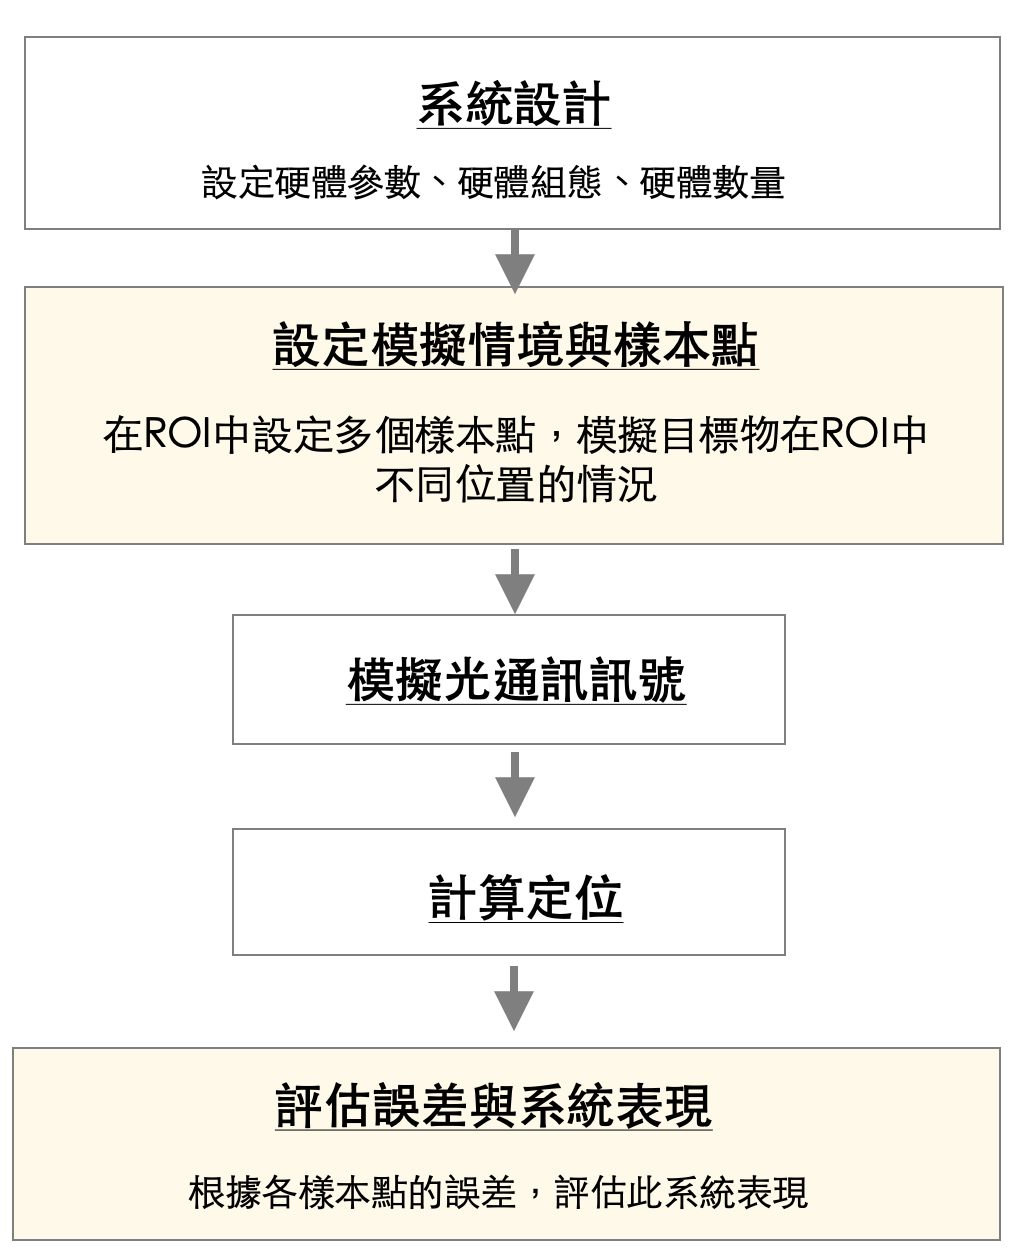
\includegraphics[width=8cm]{ch4pic/evaluate_flow.png}
    \caption{評估系統流程圖}
    \label{pic:evaluate_flow}
\end{figure}

為了針對不同使用情境評估系統表現,模擬流程整理於圖\ref{pic:simulation_flow},其中,由於在評估系統時,需要對不同的使用情境進行設計,因此我們的模擬流程由定義使用情境開始,參考\ref{chp:scenario}章,而根據不同使用情境,量測與目標單位於空間中的相對位置與姿態也會有所不同。系統設計的部分於\ref{chp:hardware_design}章中介紹,需決定的部分包含硬體數量、硬體參數以及硬體組態。有了硬體組態與座標轉換關係,即可透過式\ref{eqn:model_coor_extend}計算出相對位置,如何模擬硬體誤差則在\ref{chp:hardware_error}章中介紹。最後則是透過第三章提出的演算法,計算出相對位置與誤差。
\subsection{評估方法}
\subsubsection{使用情境與樣本點}
\subsubsection{量化系統表現}


\subsection{系統設計對系統表現的影響}
\subsubsection{硬體指向對系統表現的影響}
\subsubsection{朗博次方對系統表現的影響}
\subsubsection{硬體數量對系統表現的影響}

\subsection{不同使用情境的系統表現}


\section{結論}
\label{chp:4_conclusion}

%______________________________________




% 硬體參數的部分,LED參考\cite{datasheet:led_vsma},以供應5A時的輻射強度作參考,取$Pt=1.7\pi W$,而PD則參考\cite{datasheet:BPW},將$Re\times A = 4.2\times10^{-6}$,而兩硬體的朗博次方則都設定為一。




% \subsection{定義模擬情境}
% \label{chp:scenario}

% 為了針對不同使用情境評估系統表現,我們於此情境中的感興趣區域(Region of Interest,以下簡稱ROI)中建立多個樣本點,針對第$k$個樣本點中量測出的相對位置$\hat{^{PL}_{k}\boldsymbol{T}}$,計算出與實際相對位置$^{PL}\boldsymbol{T}$的誤差$_k e$,參考圖\ref{pic:error_show}。其中,ROI是相對PD座標系去作定義,也就是將PD視為固定,定義LED座標系相對於PD座標系的座標轉換關係$^{PL}\boldsymbol{H}$。僅定義LED座標系相對於PD座標系的關係之原因,是因為在不考慮環境障礙物情況下,兩座標系的絕對位置並不重要,僅有相對關係會對相對位置造成影響。

% \begin{figure}[ht]
%     \centering
%     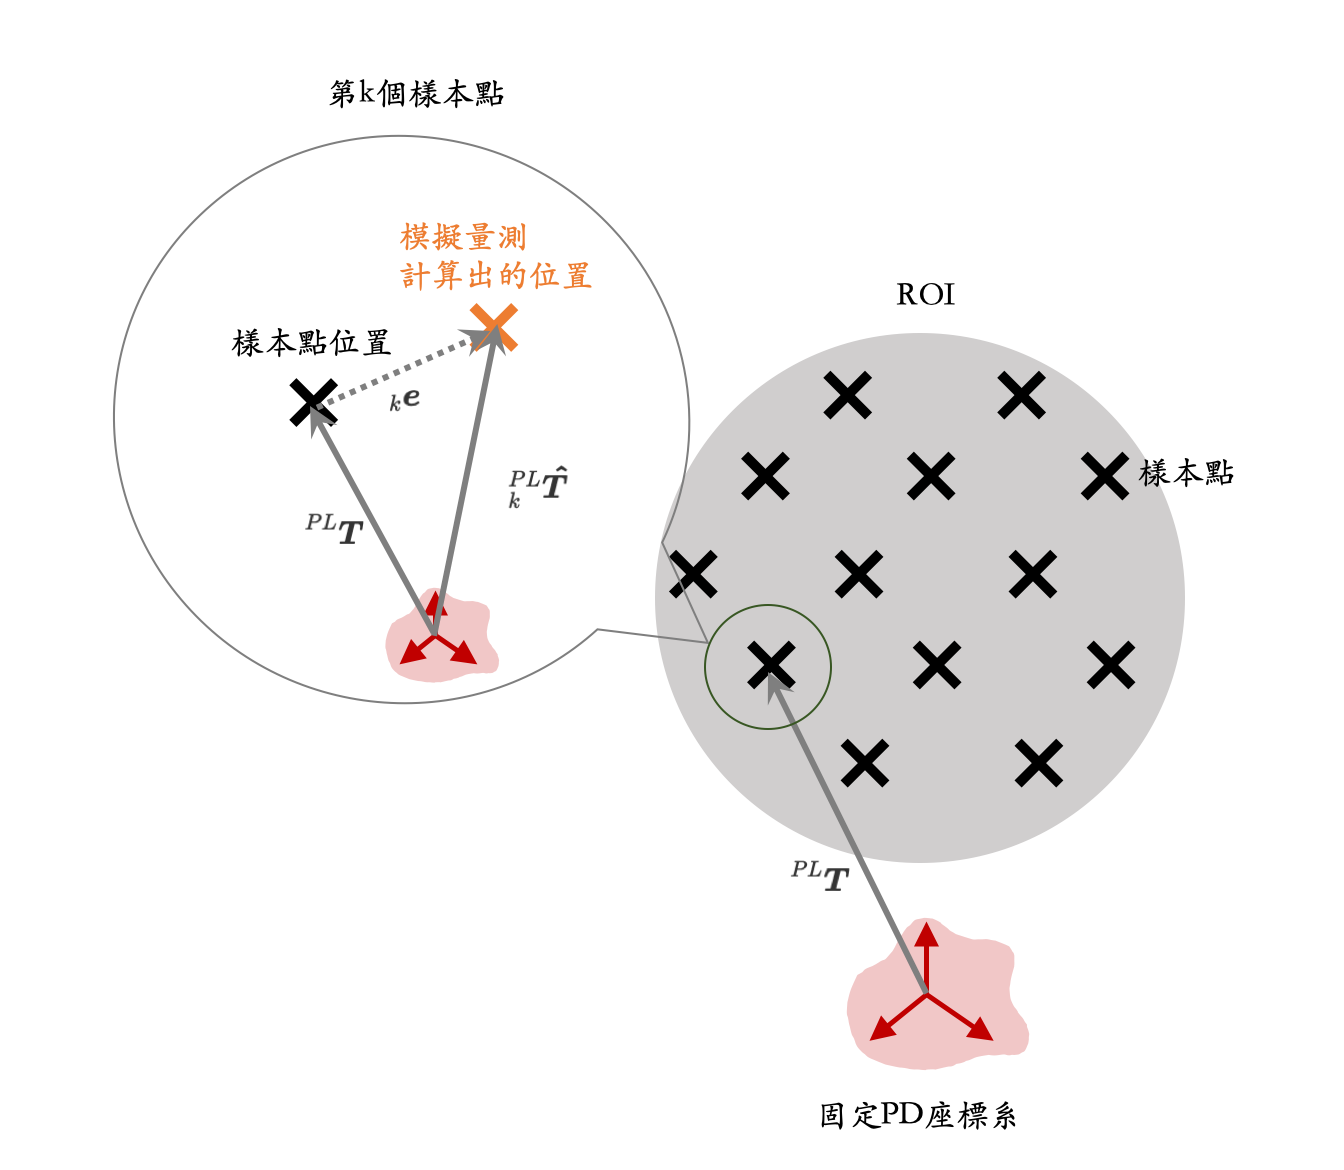
\includegraphics[width=9cm]{ch4pic/error.png}
%     \caption{樣本點與誤差}
%     \label{pic:error_show}
% \end{figure}

% 在這裡,我們選擇常見的室內定位情境作為模擬情境,也就是目標物LED座標系固定於天花板朝地面照射,而量測者的PD座標系於室內空間中,測試範圍設置的較\cite{case:cart3d}\cite{case:3d_layers}中的都大,為$3 \times 3 \times 3 m$的範圍,如圖\ref{pic:translate_sample}。而由於本研究所使用的演算法並不需限制目標平面與量測平面平行,因此兩座標系之間的姿態也可以改變,除了平移的樣本點還需建立旋轉的樣本點,旋轉樣本點由翻滾(以下稱為Roll)、俯仰(以下稱為Pitch)、偏擺(以下稱為yaw)三個旋轉角度定義,旋轉順序依序為Roll, Pitch, Yaw。旋轉樣本可參考圖\ref{pic:rotate_sample},紅色箭頭代表的是PD座標系Z軸,藍色的各個箭頭則代表與其相對的的LED座標系Z軸,並以極座標圖呈現於圖中。

% \begin{figure}[ht]
%     \centering
%     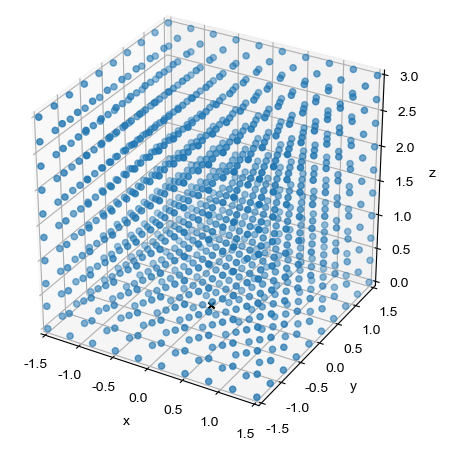
\includegraphics[width=6cm]{ch4pic/translate_sample.png}
%     \caption{平移樣本點}
%     \label{pic:translate_sample}
% \end{figure}

% \begin{figure}[ht]
%     \centering
%     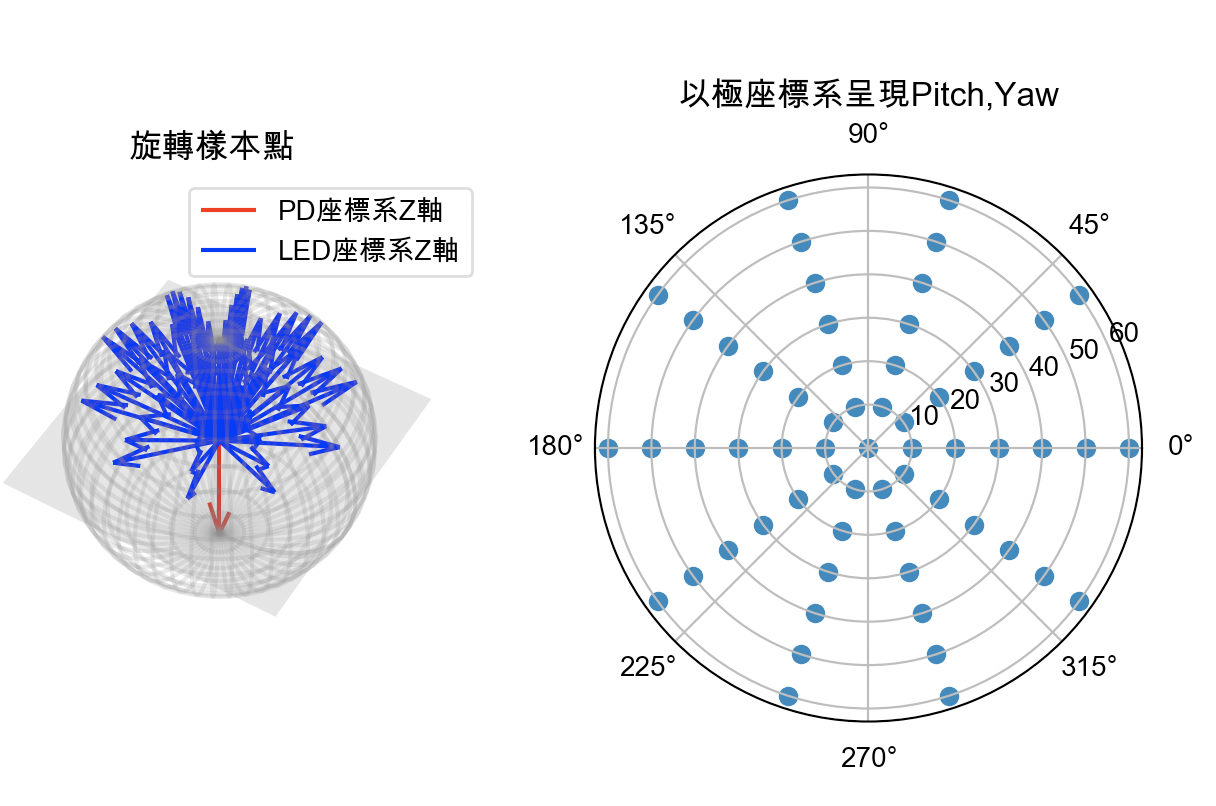
\includegraphics[width=8cm]{ch4pic/rotate_sample.png}
%     \caption{旋轉樣本點}
%     \label{pic:rotate_sample}
% \end{figure}

% \begin{table}[h!]
%     \begin{center}
%       \caption{平移樣本點}
%       \label{tab:translate}
%       \begin{tabular}{c|c|c|c} % <-- Alignments: 1st column left, 2nd middle and 3rd right, with vertical lines in between
%          & \textbf{最小值} & \textbf{最大值}&\textbf{樣本數}\\
%         \hline
%         $t_x$ & -1.5 & 1.5&10\\
%         $t_y$ & -1.5 & 1.5&10\\
%         $t_z$ & 0 & 3 &10\\
%       \end{tabular}
%     \end{center}
%   \end{table}

%   \begin{table}[h!]
%     \begin{center}
%       \caption{旋轉樣本點}
%       \label{tab:rotate}
%       \begin{tabular}{c|c|c|c} % <-- Alignments: 1st column left, 2nd middle and 3rd right, with vertical lines in between
%         & \textbf{最小值} & \textbf{最大值}&\textbf{樣本數}\\
%        \hline
%        Roll & $\pi$ & $\pi$&1\\
%        Pitch & $\pi/18$ &$\pi/3$&6\\
%        Yaw & $\pi/5$ & $2\pi$&10\\
%      \end{tabular}
%    \end{center}
%  \end{table}

% 如表\ref{tab:translate}中所示,一共有$10\times 10\times 10$總共一千個平移樣本點,旋轉樣本點則有$1\times 6\times 10$共六十個,兩者相乘代表總共六萬個樣本點。這代表著每個平移樣本點上皆需做出60次旋轉,以旋轉樣本點來看也是,每個旋轉樣本點都需在每個平移樣本點上計算一次。










% % --------------------------------------



% % --------------------------------------
% \section{評估系統表現}
% \label{chp:system_perform}



% 根據以上設定,我們將六萬個樣本點進行定位,然而,各樣本點都有可能遇到無法求解的狀況,如\ref{chp:orient_conclu}章所提到,若沒有任何一個LED同時將訊號傳送給三個以上的PD,則無法解出方位;而若沒有任何一個PD同時接受到三個以上LED資訊,則無法計算距離。即使我們今天系統設計有超過三個以上的LED與PD硬體數量,在\ref{chp:algorithm_filter}章中也會將訊號過大、過小的數值去除,導致所得訊號不足求解的狀況。在各樣本點可能會解不出來的情況下,解不出來則會完全無法計算誤差,因此無法利用樣本點平均誤差來完整描述系統的表現。

% 因此,我們改看「在容許範圍$To$(Tolerance)」內的樣本點比例,在這邊我們設定$To=0.1m$,而結果呈現於圖\ref{pic:sample_out}。

% \begin{figure}[ht]
%     \centering
%     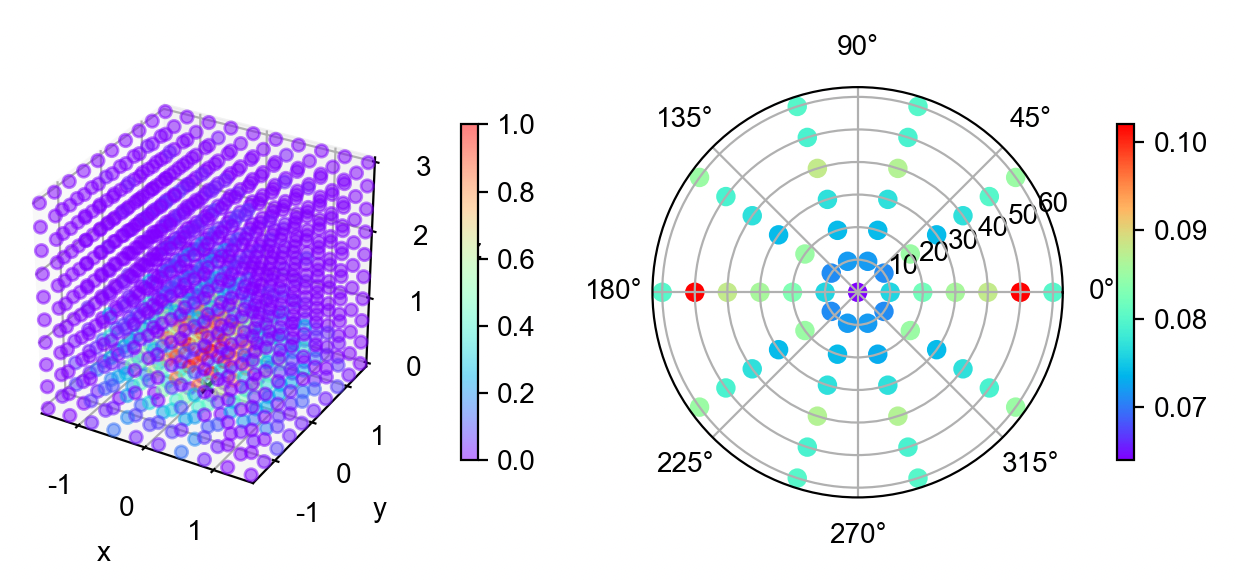
\includegraphics[width=9cm]{ch4pic/sample_out.png}
%     \caption{容許範圍內的樣本點比例}
%     \label{pic:sample_out}
% \end{figure}

% 觀察圖中的現象,在PD座標系延伸出去,有一橢圓區塊具有很高的定位能力,定位能力的分佈與其他文獻符合。

% 而由於第三章此演算法並沒有限制硬體數量、朗博次方與硬體指向,在設計上是有靈活度的,因此我們透過改變這幾項變數,來觀察系統的反應。其中,LED與PD指向的部分,我們將每個硬體皆具有的兩個由度限制剩下一個,假設方位角平均分配:$^P\beta_p = 2\pi/P$、$^L\beta_l = 2\pi/L$,仰角的部分則限制必須相同$^P\alpha_p =^P\alpha$、$^L\alpha_l = ^L\alpha$。在這樣的限制下,我們分別探討各項變數的影響。



% \subsection{朗博次方的影響}

% 在假設$^P\alpha_p =\pi/18$、$^L\alpha_l = \pi/18$,以及硬體數量$L=P-8$的情況下,我們改變朗博次方,並將樣本中於容許範圍內的比例,呈現於圖\ref{pic:m_translate}與圖\ref{pic:m_rotate}中。隨著朗博次方的提升,硬體所照射的範圍越來越小,因此容許範圍內比例高的的區域便越顯集中。

% \begin{figure}[h!]
%     \centering
%     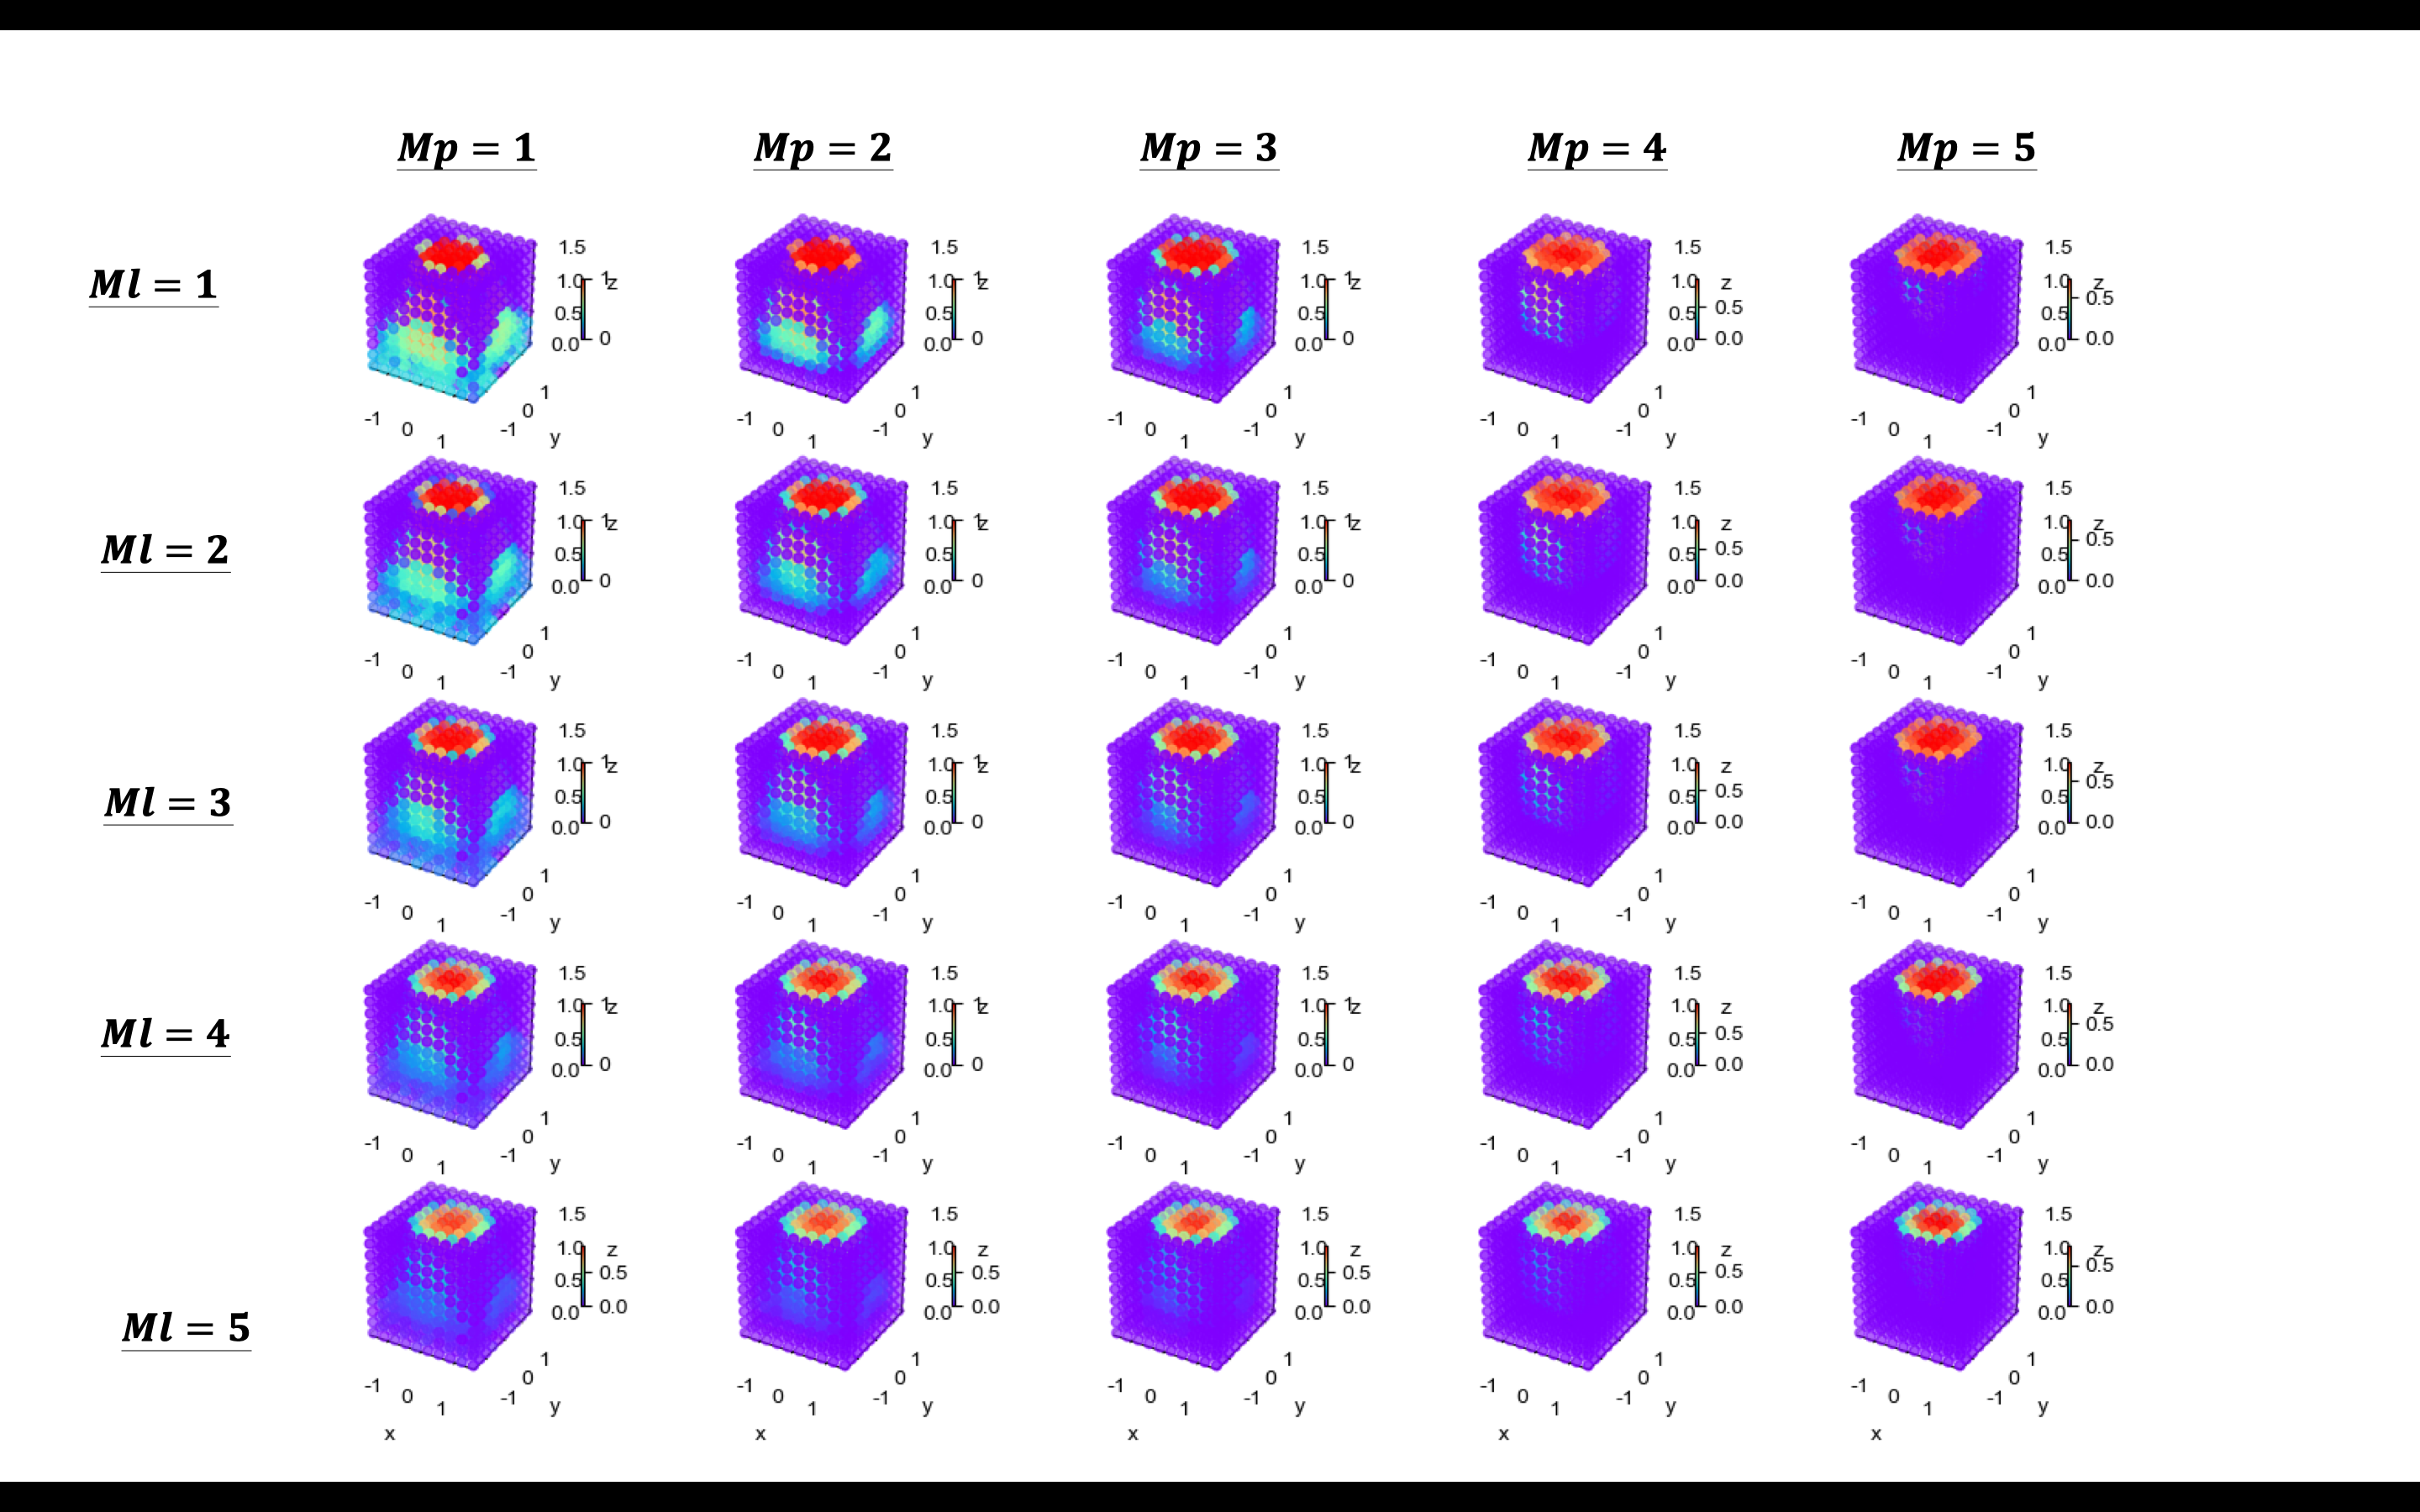
\includegraphics[width=14cm]{ch4pic/m_translate.png}
%     \caption{改變朗博次方對平移樣本點的影響}
%     \label{pic:m_translate}
% \end{figure}
% \begin{figure}[h!]
%     \centering
%     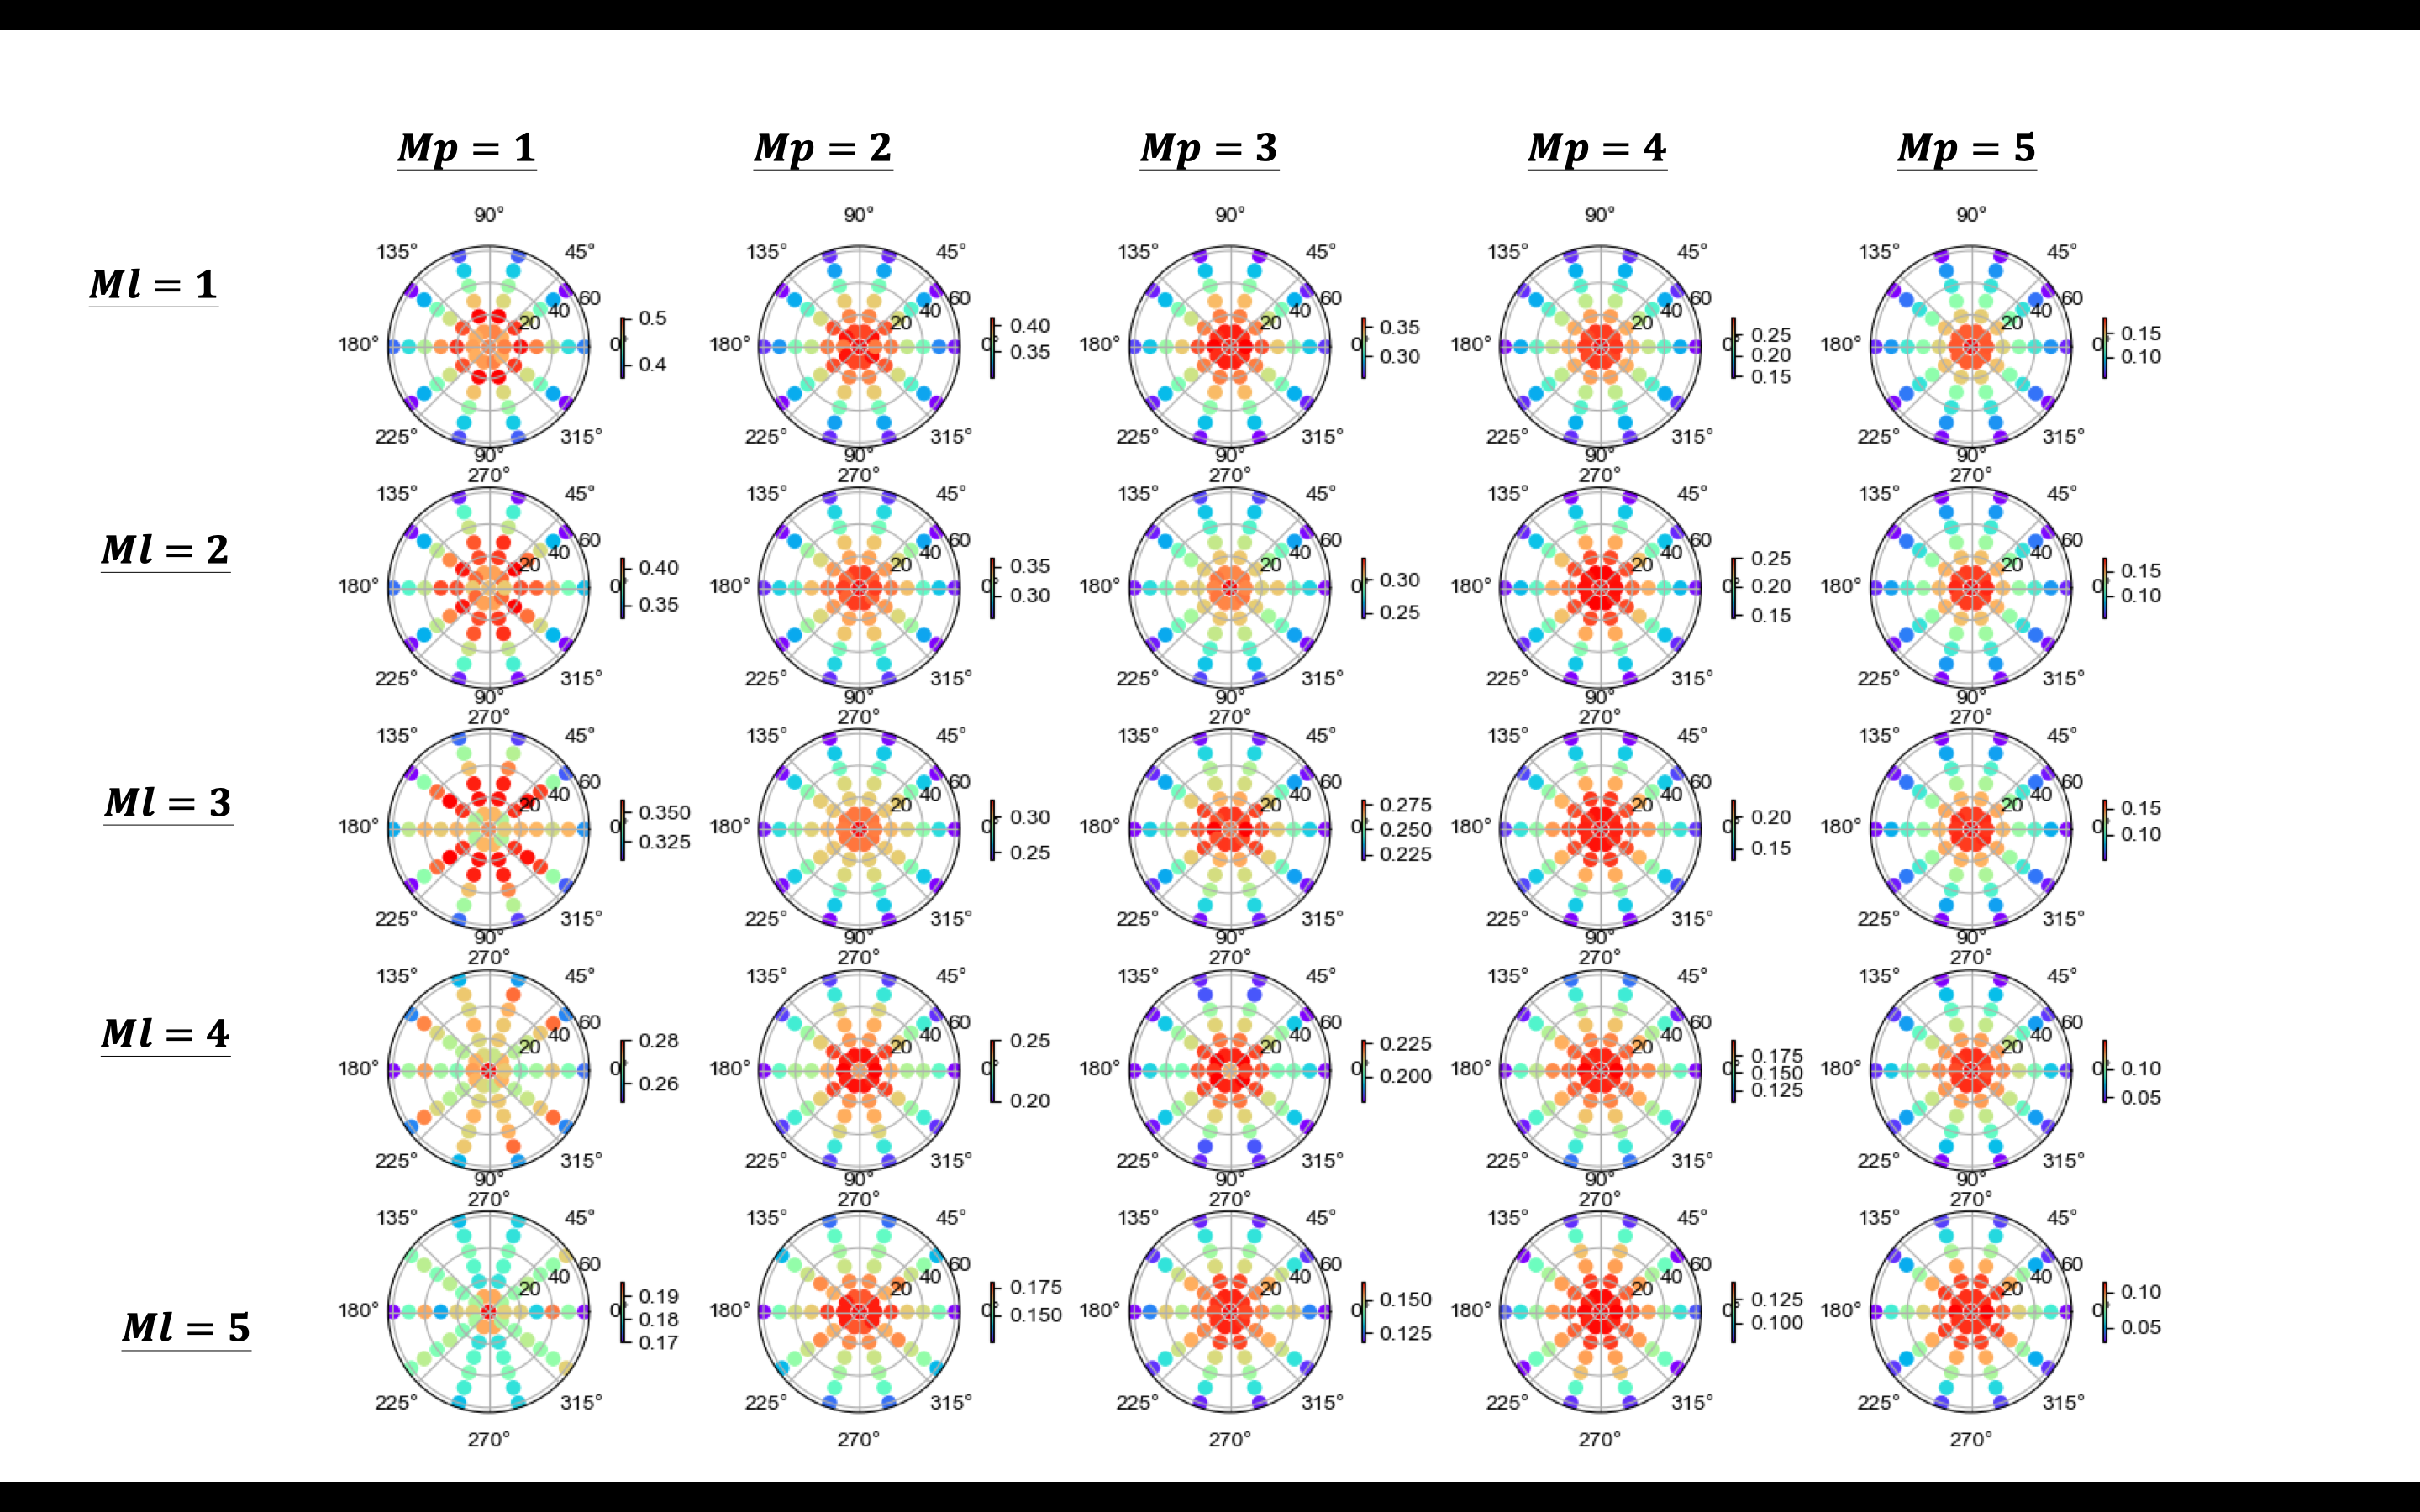
\includegraphics[width=14cm]{ch4pic/m_rotate.png}
%     \caption{改變朗博次方對旋轉樣本點的影響}
%     \label{pic:m_rotate}
% \end{figure}

% 我們將平移與旋轉樣本點總共六萬個點中,在容許範圍內的比例,呈現於圖\ref{pic:m_effect},我們可以觀察到在此情境中,較小的朗博次方使系統表現較佳。

% \begin{figure}[h!]
%     \centering
%     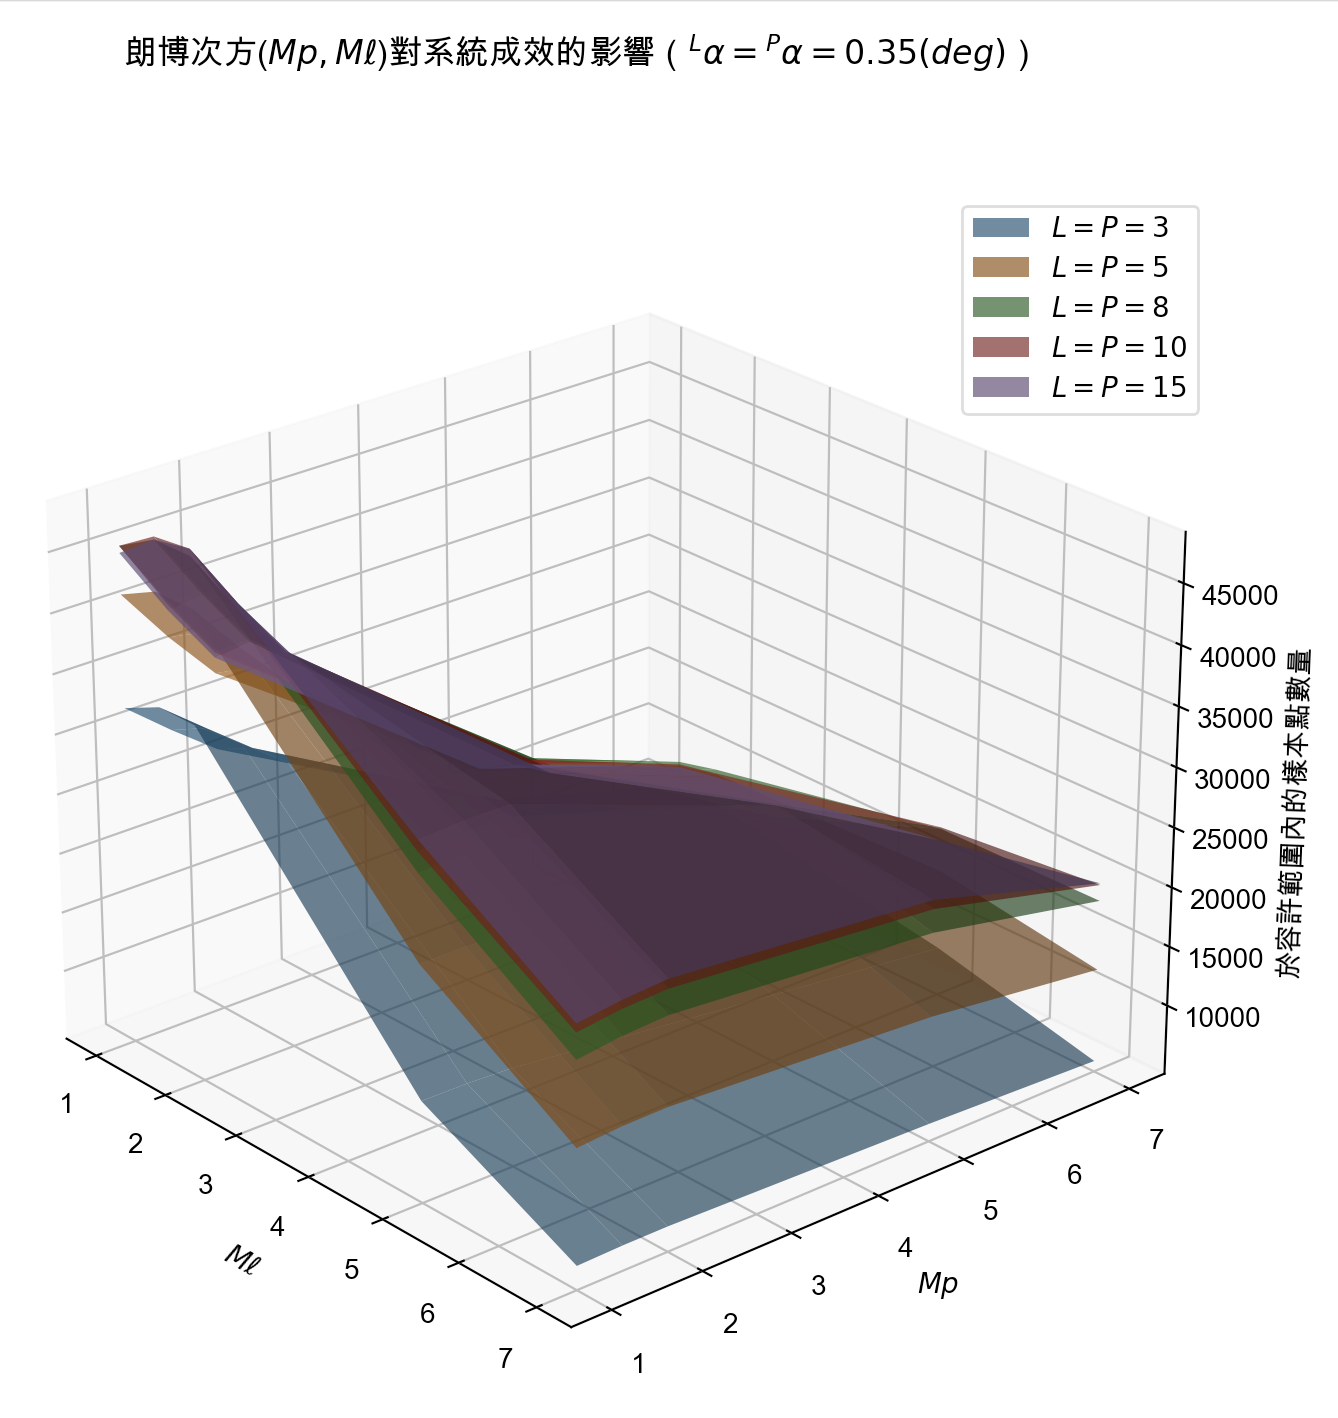
\includegraphics[width=9cm]{ch4pic/m_effect.png}
%     \caption{改變朗博次方對系統的影響}
%     \label{pic:m_effect}
% \end{figure}



% \subsection{LED與PD指向的影響}

% 在假設朗博次方$Mp=M\ell=1$,以及硬體數量$L=P-8$的情況下,我們改變硬體指向$^P\alpha,^L\alpha$,並將樣本中於容許範圍內的比例,呈現於圖\ref{pic:alpha_translate}與圖\ref{pic:alpha_rotate}中。隨著硬體指向提升,多個硬體之間重疊的覆蓋範圍便越來越小,漸漸僅剩下於中心位置的樣本點:$x,y,=0$。

% \begin{figure}[h!]
%     \centering
%     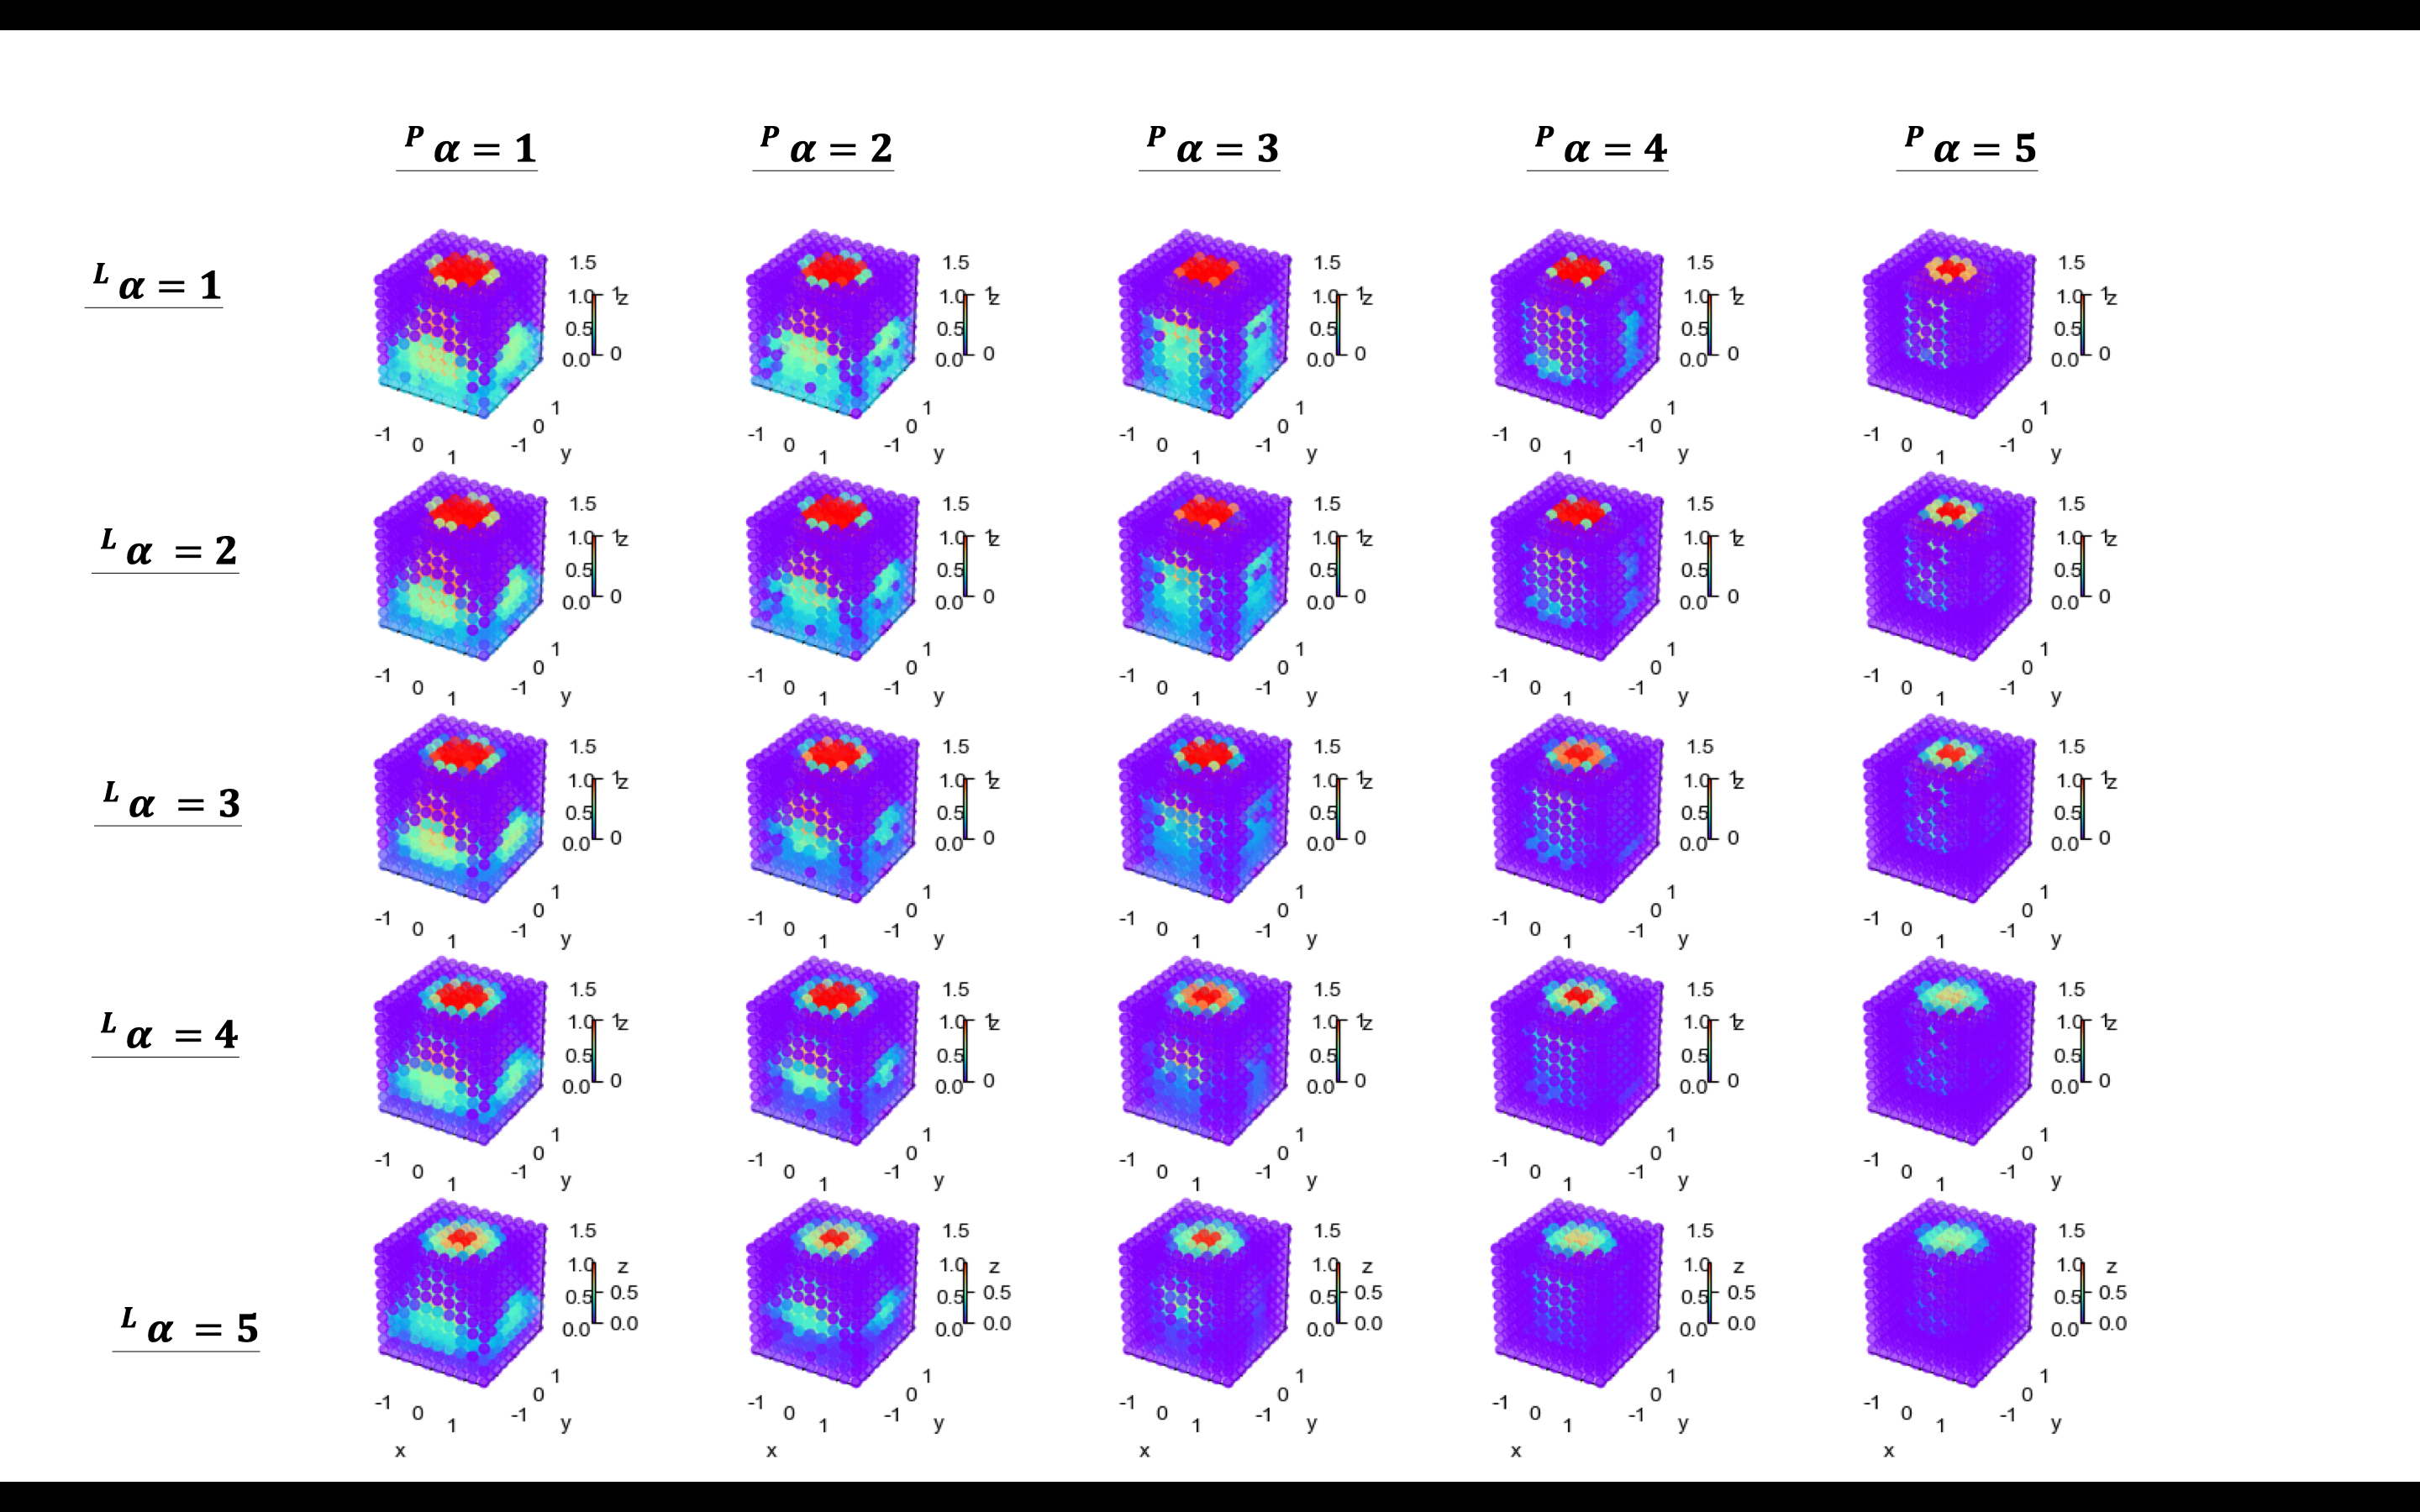
\includegraphics[width=14cm]{ch4pic/alpha_translate.png}
%     \caption{改變硬體指向對平移樣本點的影響}
%     \label{pic:alpha_translate}
% \end{figure}
% \begin{figure}[h!]
%     \centering
%     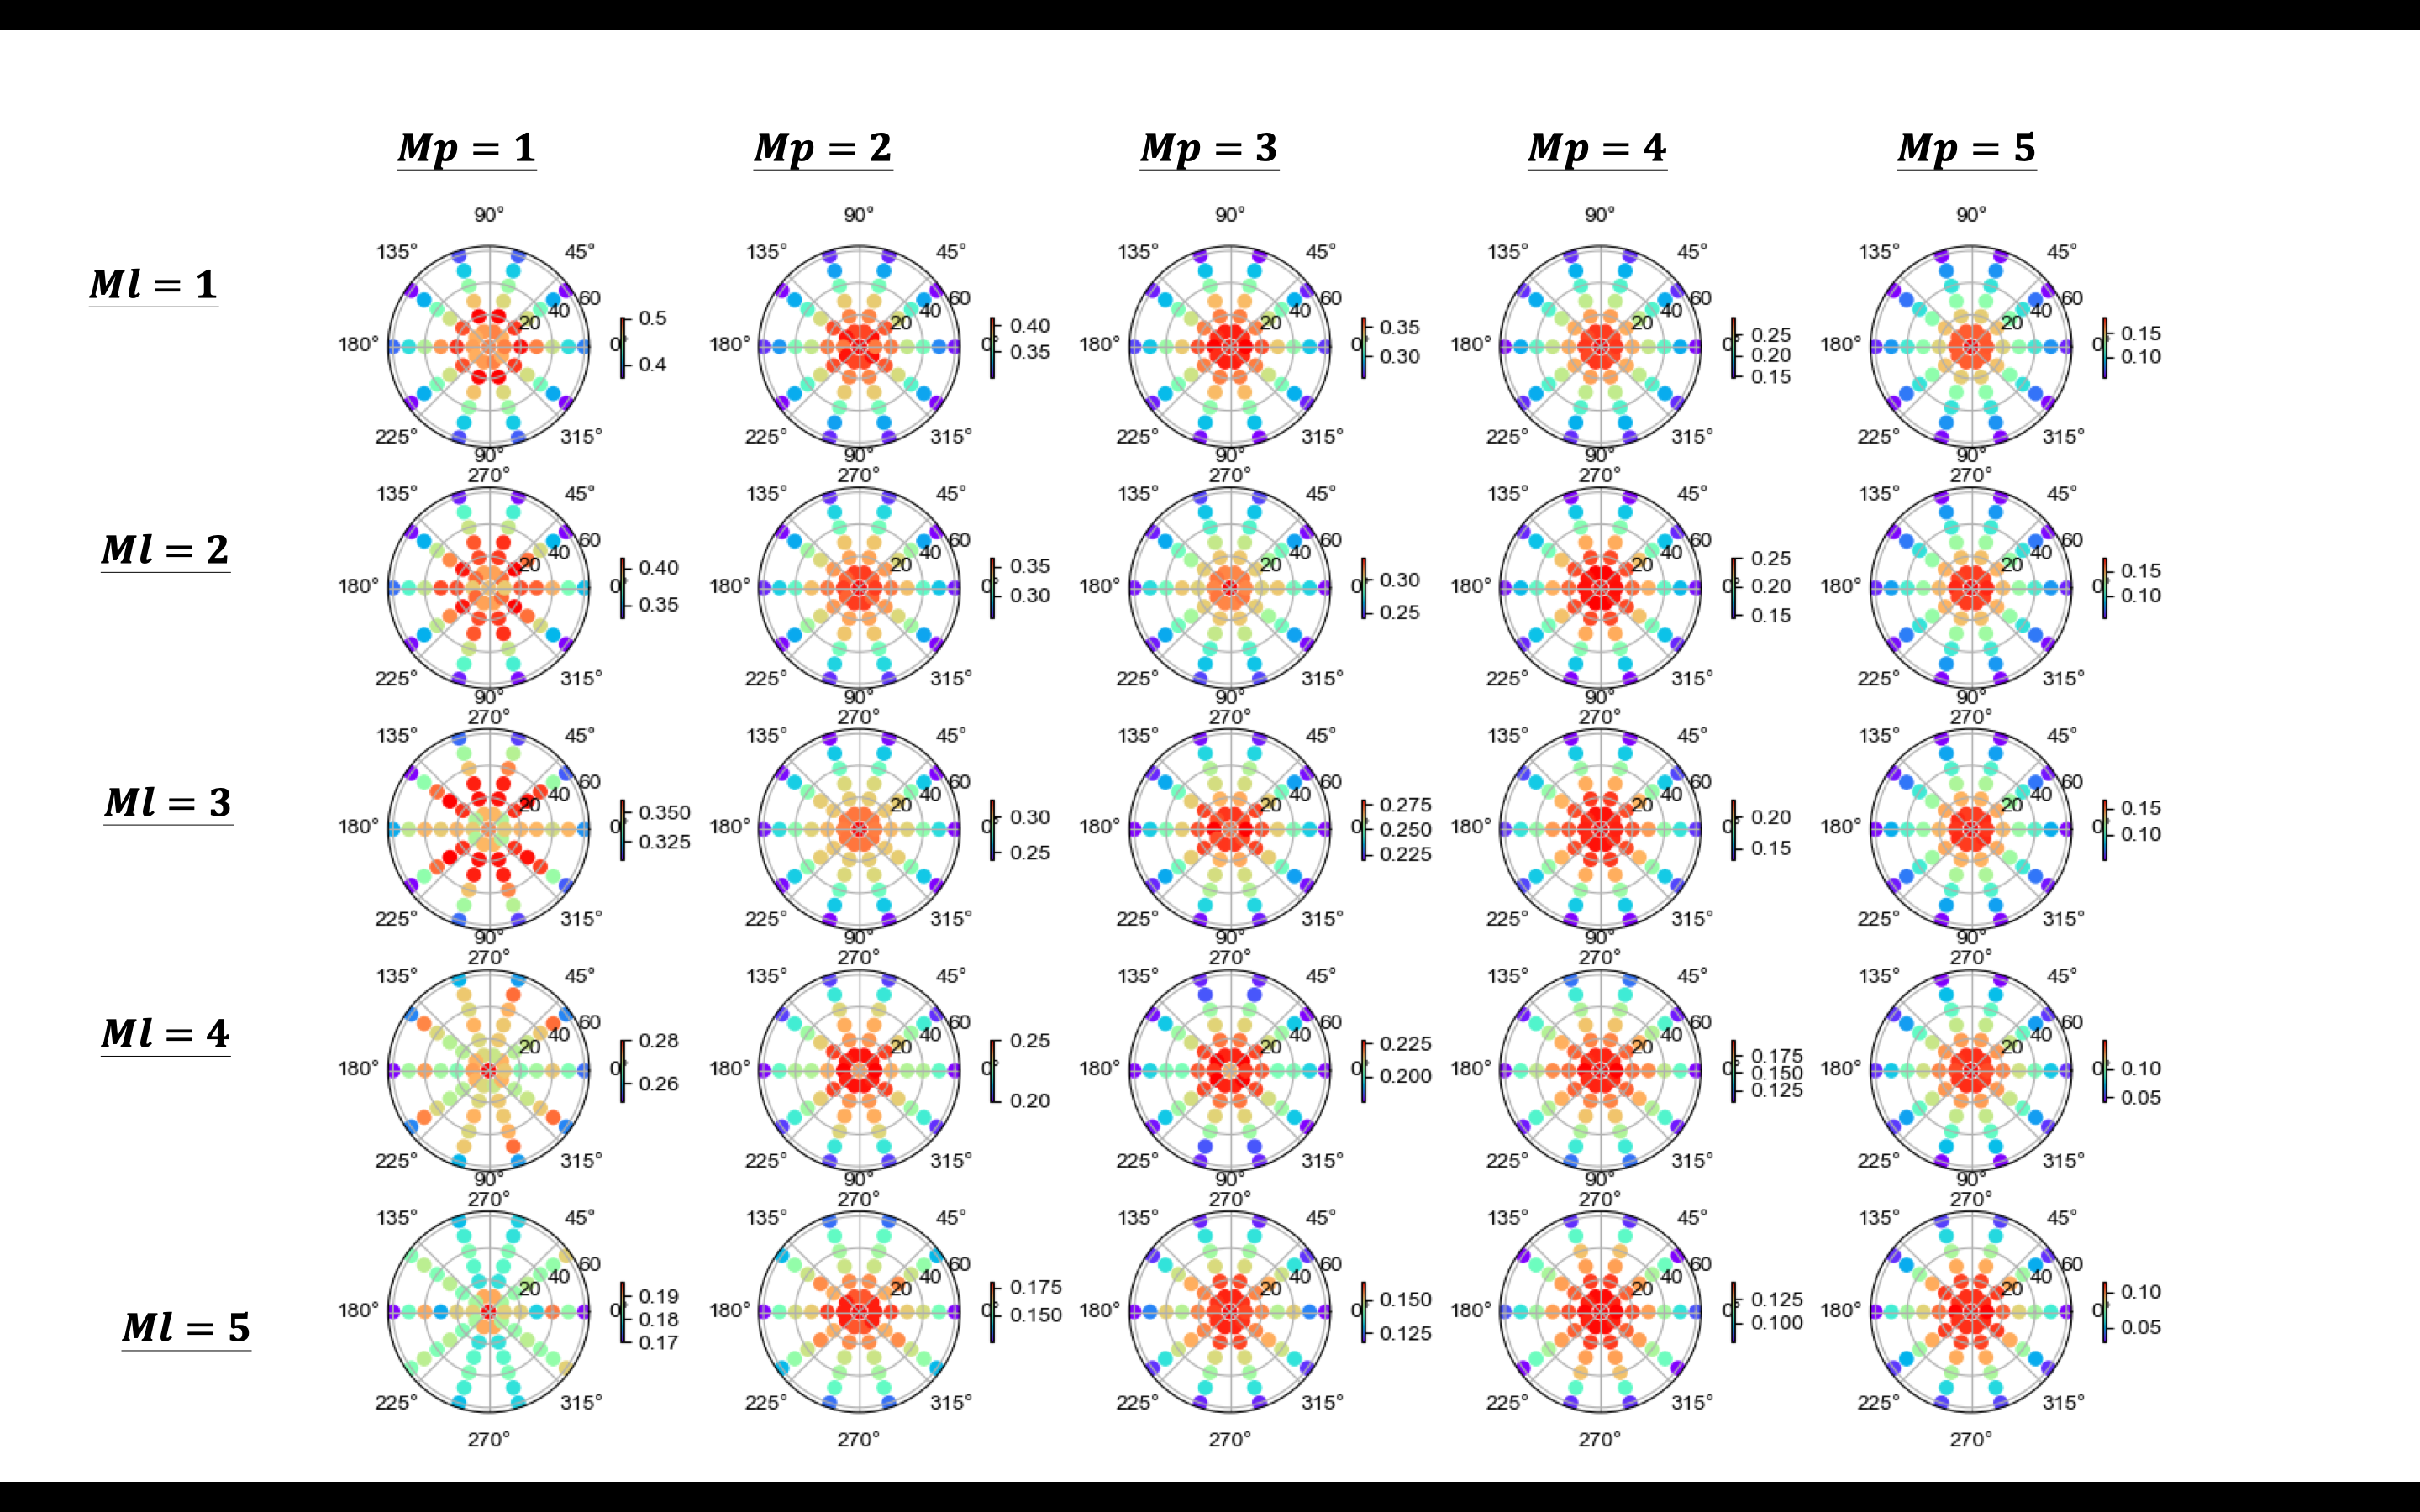
\includegraphics[width=14cm]{ch4pic/m_rotate.png}
%     \caption{改變硬體指向對旋轉樣本點的影響}
%     \label{pic:alpha_rotate}
% \end{figure}

% 我們將平移與旋轉樣本點總共六萬個點中,在容許範圍內的比例,呈現於圖\ref{pic:alpha_effect},我們可以觀察到在此情境中,較小的硬體擺設天頂角,使系統表現較佳。

% \begin{figure}[h!]
%     \centering
%     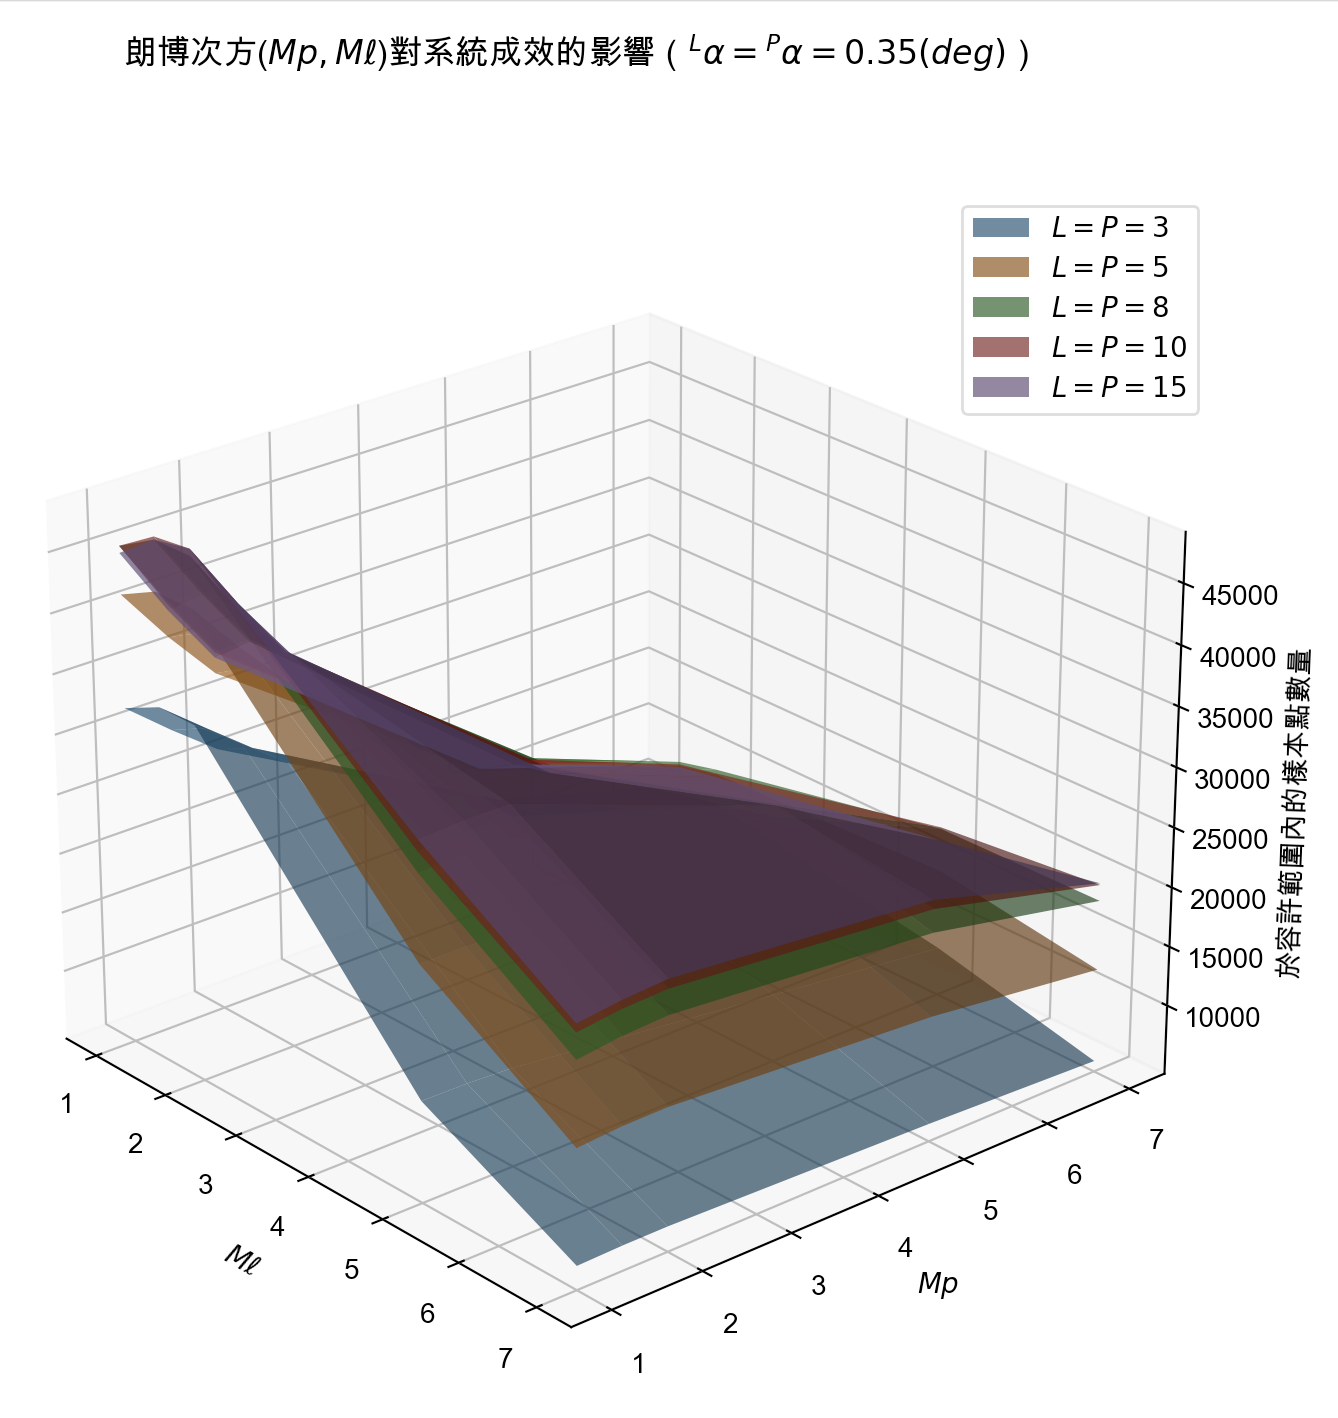
\includegraphics[width=9cm]{ch4pic/m_effect.png}
%     \caption{改變硬體指向對系統的影響}
%     \label{pic:alpha_effect}
% \end{figure}



% \subsection{LED與PD數量的影響}

% 由圖\ref{pic:m_effect}與圖\ref{pic:alpha_effect}中,我們都可以看出在提高硬體數量時,系統表現提升,然而系統表現提升的幅度不與硬體提升的數量成正比。因此,在挑選硬體數量時,除了系統表現以外,也需將硬體增加所造成的硬體成本,以及架設系統的難度考慮進來,在系統表現與硬體系統簡單中取捨。













% % --------------------------------------
% \section{結論}
% \label{chp:4_conclusion}


% 由以上分析,我們可以看出在\ref{chp:scenario}章中提出的情境下,小的朗博次方與較小的硬體天頂角$\alpha$使系統的表現較佳,而硬體數量則是愈多愈好,但成長的趨勢隨著硬體數量增多而減慢。

% 我們本章節提出的方法,可以在軟體中透過改變硬體的選擇、樣本點的集合、組態等,快速的對不同情境,評估不同系統設計的表現。有了此模擬方法,我們可以在硬體系統架設之前對系統表現有所了解,避免在硬體架設的部分浪費時間與硬體成本。除此之外,藉由可以分析不同設計下的系統表現,我們進而於第五章針對不同情境,進行朗博次方、硬體指向以及硬體數量的最佳化,提供特定使用情境下的最佳系統設計。
